%\documentclass{article}
\documentclass[conference]{IEEEtran}
\IEEEoverridecommandlockouts

% Language setting
% Replace `english' with e.g. `spanish' to change the document language
\usepackage[english]{babel}

% Set page size and margins
% Replace `letterpaper' with `a4paper' for UK/EU standard size
\usepackage[letterpaper,top=2cm,bottom=2cm,left=3cm,right=3cm,marginparwidth=1.75cm]{geometry}

% Useful packages
\usepackage{amsmath,amssymb,amsfonts}
\usepackage{graphicx}
\usepackage[colorlinks=true, allcolors=blue]{hyperref}
\usepackage{booktabs}
\usepackage{adjustbox}
\usepackage{cleveref}
\usepackage{todonotes}
\usepackage{array} % required for text wrapping in tables

\newcommand{\reminder}[2][]
{\todo[color=blue!18, #1]{#2}}

\title{Can't Gen This: A Survey on Intellectual Property Protection Methods for Data in Generative AI}
% Protecting intellectual property in the age of generative AI: A review of technical approaches and challenges 
% Guarding creativity: Technical Strategies for Safeguarding Digital Content Intellectual Property in Generative AI training
% Digital Guardians: Protecting Intellectual Property in the Generative AI Applications – A Comprehensive Survey


\author{
    \IEEEauthorblockN{Tanja Šarčević}
    \IEEEauthorblockA{\textit{SBA Research},
        Vienna, Austria\\
        tsarcevic@sba-research.org
        %, 0000-0003-0896-9193
    }
\and
    \IEEEauthorblockN{Alicja Karlowicz}
    \IEEEauthorblockA{\textit{SBA Research},
        Vienna, Austria\\
        akarlowicz@sba-research.org
        %, 
    }
\and
    \IEEEauthorblockN{Rudolf Mayer}
    \IEEEauthorblockA{\textit{SBA Research},
        Vienna, Austria\\
        rmayer@sba-research.org
        %, 0000-0003-0424-5999
    }
\and
    \IEEEauthorblockN{Ricardo Baeza-Yates}
    \IEEEauthorblockA{\textit{Northeastern University},
        Boston, MA, USA\\
        ricardo.baeza@upf.edu
        %, 0000-0003-3208-9778
    }
\and
    \IEEEauthorblockN{Andreas Rauber}
    \IEEEauthorblockA{\textit{TU Wien},
        Vienna, Austria\\
        andreas.rauber@tuwien.ac.at
        %, 0000-0002-9272-6225
    }
}

\begin{document}
\maketitle
\thispagestyle{plain}
\pagestyle{plain}

\begin{abstract}
Large Generative AI (GAI) models have the unparalleled ability to generate text, images, audio, and other forms of media that are increasingly indistinguishable from human-generated content.
%This generated content is synthesised from great volumes of human-made artefacts exhibiting familiar patterns.
% give an impression of the ability to produce original and creative content provided abstract human description. However, this is hardly the case because these outputs are in fact created by combining fragments of human-made artefacts arranged in familiar patterns learned from great volumes of data. 
As these models often train on publicly available data, including copyrighted materials, art and other creative works, they inadvertently risk violating copyright laws and misappropriating intellectual property.
Due to the rapid development of generative technology and pressing ethical considerations from stakeholders, protective mechanisms and techniques are emerging at a high pace but lack a systematisation.

In this paper, we study the concerns regarding the intellectual property rights of training data and specifically focus on the properties of generative models that enable misuse leading to potential IP violations. We further provide a systematic review of technical solutions for safeguarding the data from intellectual property violations in GAI.

  
% We hope to contribute to the ongoing conversation about the complex relationship between technology, creativity, and legal rights in the age of generative AI. We discuss the importance of addressing these challenges proactively, with a goal of balance between AI-driven innovation and the protection of intellectual property rights.
\end{abstract}

\section{Introduction}
Generative Artificial Intelligence (GAI) has revolutionised various domains, demonstrating remarkable capabilities in generating realistic images~\cite{rombach_high-resolution_2022,ramesh_hierarchical_2022}), %noauthor_dalle2_nodate}), 
text~(ChatGPT~\cite{openai_gpt-4_2023}) and music~(MuseNet\footnote{\url{https://openai.com/research/musenet}}). %~\cite{noauthor_musenet_nodate} 
This cutting-edge technology has the potential to disrupt traditional creative processes, enabling AI systems to autonomously produce content that mirrors human creativity. 
While GAI opens up exciting opportunities for innovation and artistic expression, it also presents significant challenges concerning intellectual property rights and ethical considerations.
\begin{figure}[ht]
    \centering
    \includegraphics[width=\linewidth]{figures/teddy.png}
    \caption["\textit{A photo of a teddy bear on a skateboard in Times Square.}" by DALL-E 2]{"\textit{A photo of a teddy bear on a skateboard in Times Square.}" by DALL-E 2\footnotemark.
    %~\cite{noauthor_dalle2_nodate}     
    } 
    \label{fig:enter-label}
\end{figure}
\footnotetext{\url{https://openai.com/dall-e-2}}
Intellectual property rights (IPR) encompass a set of legal protections designed to safeguard the creations of human intellect. These rights, including copyright, patents, trademarks, and trade secrets, have played a vital role in promoting creativity, innovation, and fair compensation for creators. However, the emergence of GAI has sparked debates surrounding the nature of these rights when AI systems generate original content without direct human intervention but rather by generalising from a large corpus of human creation.

Recently, artists have been noticing the evidence of the non-originality of generative models through some controversial examples. 
The name of a Polish artist, Greg Rutkowski, known for his fantasy illustrations, appeared in more than 93,000 prompts of Stable Diffusion - the prompts have been used to create art in his distinct style, very successfully so. 
As a result, many AI-created images inspired by Rutkowski's style have been published and appear in online searches~\cite{mit_technology_review_this_2022}. The case was followed by more artists reporting the same behaviour of generative models. 
Three artists, Sarah Anderson, Kelly McKernan, and Karla Ortiz filed a class action lawsuit against Stability AI\footnote{\url{https://stability.ai/}}, Midjourney\footnote{\url{https://www.midjourney.com/}}%~\cite{noauthor_midjourney_nodate}
, and Deviant Art\footnote{\url{https://www.deviantart.com/}}%~\cite{noauthor_deviantart_nodate}
, over their usage of Stable Diffusion~\cite{rombach_high-resolution_2022}, alleging copyright infringement. They assert that these models used their works and the works of thousands of other artists as training data without authorisation.
Another lawsuit was filed by Getty Images against Stability AI for using more than 12 million images and associated metadata without authorisation or compensation to train their model~\cite{nolan_ai_2023}.

One major aspect of the underlying problem and an aspect that distinguishes these current from historic cases of plagiarism and other forms of copyright infringement is the sheer scale.
While the artists take years of education and practice to develop their distinct artistic style and ultimately profit from commissioning their art, tools that use their art without consent and create a competitive alternative in an instant and seemingly without a quantitative limit present a threat to their work and careers.

This situation sparked research on mitigation methods for potential intellectual property rights violations in GAI. 
The protection encompasses a diverse array of technical strategies, each tailored to address specific vulnerabilities.
For instance, some techniques aim to support the artist in opting out of large scraped datasets, while other works focus on disabling style mimicry behaviours. 
Many of these techniques build upon prior research on other ethical issues in GAI, such as privacy~\cite{matsumoto_membership_2023} 
and inappropriate content generation~\cite{gandikota_erasing_2023}.

We have now arrived at a point where a multitude of technical solutions are available, but a systematisation of the threats and vulnerabilities they address, their costs (e.g. in terms of distorting original artwork), and their shortcomings for protection is lacking.
This paper addressed this gap. It systematically reviews the current state-of-the-art technical approaches for safeguarding training data against copyright and IP violations. 
We outline the potential violations of intellectual property considered in the literature and provide a discussion about the underlying properties of generative models that enable such violations. 
Following this, we present a variety of technical strategies, ranging from training data sanitisation, model modifications, adversarial injections and policy-driven frameworks, that have been proposed to address these concerns.  

% This paper delves into the complex intersection of generative AI and intellectual property violations.
% We define the potential violations of intellectual property considered in the literature. 
% Further, we explore and systematise state-of-the-art technical approaches designed to mitigate IPR violations in AI-generated content. 
% Moreover, we address the ethical dilemmas arising from AI models trained on copyrighted or proprietary data, leading to concerns about ownership and attribution.


% Our contributions:
% todo



% \textit{These (alt text in english) descriptions of the images are useful for people with visual impairments who use screen reader software, and they help search engines rank the images as well. This also makes them easy to scrape, and the AI model knows which images are relevant to prompts.} ~\cite{noauthor_this_nodate}

% - Types of generative models: explain diffusion, transformers, GANs... Diffusion models feature diffusion process which converts samples from a Gaussian noise distribution intro samples from an arbitrary and more complex distribution, e.g. the distribution of natural images. This is why the SOTA techniques for image generation are indeed diffusion models. 
% Denoising Diffusion Probabilistic Models [33]1
% are
% conceptually simple: they are nothing more than image denoisers.
% Some diffusion models are further conditioned to generate a particular type of image. Class-conditional diffusion models take as input a class-label (e.g., “dog” or
% “cat”) alongside the noised image to produce a particular class of image. Text-conditioned models take this one
% step further and take as input the text embedding of some
% prompt (e.g., “a photograph of a horse on the moon”) using a pre-trained language encoder (e.g., CLIP [54]).

% % Here I can write about types of IP violations, i.e. stealing the content, mimicing -- still, maybe this can be part of the introduction
% % Furthermore, we state the properties of different models that lead to possibility of IP violation
% Contributions:
% \begin{itemize}
%     \item systematisation of mitigation techniques (we borrow some concepts aimed at mitigation of other risks, such as privacy, fake or harmful data etc.)
% \end{itemize}
This paper is organised as follows: \Cref{sec:related-work} describes other survey papers discussing the intersection of intellectual property rights and GAI. In \Cref{sec:methodology}, we describe our research methodology. In \Cref{sec:background}, we provide a detailed background on the technology underlying large generative models while in \Cref{sec:IPR-threats} we discuss the threats to IPR in GAI applications. In \Cref{sec:mitigation} we provide taxonomy and systematisation of the state-of-the-art on protecting the IP of training data. 
In \Cref{sec:discussion} we discuss the surrounding landscape of issues in GAI and IP protection. Finally, we provide conclusions in \Cref{sec:conclusion}.

% \paragraph{Further considerations}
% \begin{itemize}
%     \item A US court judge recently overruled the copyright claim for the AI-generated image\url{https://www.theverge.com/2023/8/19/23838458/ai-generated-art-no-copyright-district-court}
%     \item The Guardian has blocked Chat GPT from scraping its content due to intellectual property considerations of the authors. 
%     \item \href{Google made a watermark for AI images that you can't edit out}{https://www.theverge.com/2023/8/29/23849107/synthid-google-deepmind-ai-image-detector}, \href{another article}{https://www.forbes.com/sites/jenniferhicks/2023/08/31/google-launches-tool-that-detects-ai-images-in-effort-to-curb-deepfakes/}
%     \item Can we use legal frameworks for human art plagiarisation and apply to the generated content?
%     \item Spawning - opting out and criticism: \url{https://techcrunch.com/2023/05/03/spawning-lays-out-its-plans-for-letting-creators-opt-out-of-generative-ai-training/}
%     \item Identifying generated content: \url{https://docs.thehive.ai/docs/ai-generated-media-recognition}
%     \item Are you copying my model? (\url{https://arxiv.org/abs/2305.10036})
%     \item The false promise of imitating proprietary LLMs (\url{https://arxiv.org/abs/2305.15717})
%     \item IBM AI forensics: \url{https://research.ibm.com/blog/AI-forensics-attribution} - and much more from IBM
%     \item a group led by Hugging Face and the AI-security startup Robust Intelligence, launched an attribution challenge last year to spur new research in an emerging field called AI attribution.
%     \item \url{https://www.linkedin.com/pulse/protect-your-ip-against-generative-ai-joel-goobich/}
%     \item Protecting prompts: \url{https://paperswithcode.com/paper/protect-your-prompts-protocols-for-ip}
%     \item BBC is blocking scraping: \url{https://www.theverge.com/2023/10/6/23906645/bbc-generative-ai-news-openai}
% \end{itemize}

\section{Related work}\label{sec:related-work}
% todo: can be placed at the end --> see comments further in the doc
% comparison with existing surveys
Several works have investigated issues surrounding IP rights in the age of GAI from different perspectives.
Surveys regarding the general issues of GAI, such as privacy and security, mention and describe methods for IP protection from the technical perspective, however, not in sufficient detail. Wang et al.~\cite{wang_survey_2023} focus only on watermarking methods in terms of IP protection. Chen et al. in two consecutive surveys~\cite{chen_pathway_2023,chen_challenges_2023} do not contain a fine-grained classification.
Wang et al.~\cite{wang_security_2023} address many relevant methods such as \textit{concept removal} from the perspective of toxic content removal, while we take a training data IP protection angle.
Zhong et al.~\cite{zhong_copyright_2023} is an empirical review that evaluates three methods for IPR protection of GANs; adversarial-based, watermarking and attribution. 

A few survey papers take a legal~\cite{smits_generative_2022,chesterman_good_2023} and societal~\cite{hristov_artificial_2020} perspective on IPR, but do not address technical protection methods. 

% \paragraph{Generative AI and Intellectual Property Rights by Smiths and Borghuis~\cite{smits_generative_2022}}
% What are the copyrights for generated content and who possesses the authorship - discussion from legal perspective. It is more about protecting the generated content rather than the owners of the training data samples. It's a higher level, legal and philosophical discussion rather than technical.
% \paragraph{Artificial Intelligence and the Copyright Survey~\cite{hristov_artificial_2020}}
% Questionnaire type of survey about the impact of AI on Intellectual property. Questions included opinions on the importance of copyright protection as an incentive to make their work available for example. 

% \paragraph{Good Models Borrow, Great Models Steal: Intellectual Property Rights and Generative AI by Chesterman~\cite{chesterman_good_2023}}
% Legal and philosophical questions: (i) Should data owners be compensated for being scraped? and (ii) should anyone and if so, who should, own the output of the generative AI? No technical protection methods.
% \paragraph{Copyright Protection and Accountability of Generative AI: Attack, Watermarking and Attribution~\cite{zhong_copyright_2023}}
% This work addresses IPR protection methods for GANs and training image data. 
% It empirically evaluates 3 methods; one based on adversarial noise (similar to or even the same as cloaking), watermarking and attribution.


\section{Methodology}\label{sec:methodology}
% todo: literature search methodology, inclusion and exclusion criteria, stats and timelines
% exclusion: works that do not evaluate on IP protection scenario are excluded, but those that describe similar or same mechanisms but in other scenarios such as privacy and harmful content removal are mentioned in section xy
\begin{figure}
    \centering
    \includegraphics[width=\linewidth]{figures/stats.png}
    \caption{The literature distribution over types of protection methods and year of publication. *Our research is expanded by various other sources, such as AI provider reports, that are highly relevant in the IP protection domain.}
    \label{fig:stats}
\end{figure}
This paper focuses on technical approaches for safeguarding the intellectual property of data used to train the generative models, such as LLMs, GANs and diffusion models. 
Issues relating to the intellectual property and copyrights of training data in a large part intersect with related ethical issues such as privacy and generation of harmful content, hence many solutions use similar ideas to achieve separate goals. We hence focus our scope on the methods that directly evaluate at least one IP violation scenario. 

%literature search .


Our literature research is based on systematic literature studies principles, following the guidelines by Kitchenham et al. \cite{kitchenham_guidelines_2007} and Wohlin \cite{wohlin_guidelines_2014} to generate the collection of peer-reviewed conference papers and journal articles (\textit{formal literature}), as well as and pre-prints of methods that also provide open-source code of their solutions (\textit{grey literature}). 
The reason for the inclusion of grey literature is the high pace of the field and the fact that many influential works might be currently under review at formal publishing venues. \Cref{fig:stats} shows the distribution of the publications of protection methods and their publication year. 
We also mention other forms of grey literature, such as blogs and articles, if they serve as technical reports of highly relevant techniques.  

%-- There is a significant bias of the protection techniques towards (i) diffusion models and (ii) image training data. % todo insert figures



\section{Background}\label{sec:background}
% todo: types of generative models, huge scraped datasets, retrieval methods (CLIP and co.) 
In this section, we describe the required background and state-of-the-art of large GAI models.

\subsection{Variational Autoencoders}
Variational Autoencoders (VAEs)~\cite{kingma_auto-encoding_2022} are a type of probabilistic generative model composed of an encoder and decoder trained together. The encoder transforms the input to lower-dimensional latent space, while the decoder reconstructs the input from this compressed representation. Unlike conventional Autoencoders, which learn a deterministic mapping from the input to the latent space, VAEs introduce probabilistic modelling, as the input space is mapped to a probability distribution. This way, VAEs express not just single points in the latent space, but distributions of potential representations. Because the latent space is continuous, the decoder can generate novel data points that smoothly interpolate among training data points. 
VAEs are optimised using both reconstruction loss, which minimises the dissimilarity between original and reconstructed data, and regularisation loss. The regularisation loss, in the form of the Kullback-Leibler divergence, ensures a balanced distribution of latent representations, preventing overfitting and encouraging the encoder to map the latent space close to a Gaussian distribution. 
VAEs are flexible in the type of data they process and can be combined with other generative models~\cite{bao_cvae-gan_2017, pandey_diffusevae_2022}.


\subsection{Generative Adversarial Networks}
Generative Adversarial Networks (GANs), introduced by Goodfellow et al.~\cite{goodfellow_generative_2014} in 2014, consist of two competing networks: the generator and the discriminator. The generator generates novel output (primarily researched are images) from the data distribution, by transforming sampled noise vectors. During the training process, the generator learns the mapping of latent space (sampled vectors) to the target data distribution.
Simultaneously, a discriminator network is trained to differentiate between samples generated by the generator and original images. The generator, in response, adjusts its parameters to fool the discriminator into accepting its outputs as authentic representations, improving its ability to produce realistic samples. Through this adversarial training, both networks compete with each other to strike a balance between their performance and produce high-quality samples. 
% also mention state-of-the-art StyleGAN and BigGAN that produce high-fidelity and high-resolution images
Since the introduction of GAN, many variations and implementation improvements have emerged resulting in notable architectures such as BigGAN~\cite{brock_large_2019}, StyleGAN~\cite{karras_style-based_2019}, or CycleGAN~\cite{zhu_unpaired_2020}, reaching state-of-the-art performance on image translation and generation tasks. 

\subsection{Diffusion Models}
%include latent diffusion by Rombach
Diffusion models, inspired by non-equilibrium thermodynamics, are based on the idea of iteratively destroying an input image and training a network to reverse this process. The concept dates back to 2015 when Sohl-Dickstein introduced the baseline idea~\cite{sohl-dickstein_deep_2015}. However, it was not until Ho et al.~\cite{ho_denoising_2020} and Dhariwal and Nichol~\cite{nichol_improved_2021} improved upon the architecture and implementation that diffusion models gained widespread recognition, later proving their utility and advantages over GANs~\cite{dhariwal_diffusion_2021}.
In the forward diffusion process, the model gradually adds Gaussian noise to the input image until it becomes pure noise. Conversely, in the reverse process, the model predicts and removes the added noise in a similar, gradual way. At inference time, the model samples from a Gaussian distribution and performs denoising to generate a novel image.

Diffusion models suffer from high computational complexity and long inference time. Latent diffusion models (LDMs) address this issue by operating in the latent space rather than directly in the pixel space~\cite{rombach_high-resolution_2022}. Transforming the images into latent representations compresses the data into lower-dimensional forms, which are perceptually equivalent, yet they reduce the complexity of the input and preserve the details in the decoded images.
In LDMs, the encoding and decoding processes are handled separately from the diffusion process. An independent autoencoder is utilised for this purpose. The autoencoder is trained to transition between latent representations and images using perceptual loss to compare high-level features and patch-based adversarial objectives to capture finer details and enhance realism. 
Additionally, a regularisation term is added, similar to standard VAEs, in order to prevent high-variance latent representations, by pushing them towards Gaussian distribution. 
Consequently, during the inference phase, LDMs generate a latent representation, which is then translated into a high-quality image by the decoder.

Generation via diffusion models can be conditioned on image labels or complex text prompts semantically describing the desired output image. Text-to-image models utilise text encoders such as Contrastive Language-Image Pre-Training (CLIP)~\cite{radford_learning_2021} to capture the natural language of text prompts and map it to embeddings later injected into the model.

\subsection{Large Language Models}
% which models make sense to mention?? - look which ones are mentioned later
While the models described above are mostly used for image generation, the rise of GAI fueled by Large Language Models (LLMs) has opened new horizons for text generation. LLMs are general-purpose language models trained on extensive text datasets crawled from the Internet. They typically rely on self-attention and transformer-based architecture~\cite{vaswani_attention_2017} to predict the next token in a sequence and allow to capture long-context dependencies in text. The interaction with LLMs is commonly done through prompt engineering, where users provide specific instructions to the model. LLMs are versatile and can be used for a variety of tasks such as text generation, translation, summarisation, and question-answering. Notable models include the family of Generative Pre-trained Transformers (GPTs) from OpenAI~\cite{radford_improving_nodate, openai_gpt-4_2023}, with GPT-3.5 featured in the popular ChatGPT chatbot. Recent advancements in LLMs encompass diverse models such as the Gemini model family~\cite{gemini_team_gemini_2023}, Large Language Model Meta AI (LLaMA)~\cite{touvron_llama_2023}, and StableLM\footnote{\url{https://stability.ai/stable-lm}}, developed by Stability AI.
% gpts, palm, gemini, llama

\section{Threats to the IP of training data in GAI}\label{sec:IPR-threats}
In this section, we first enumerate the potential IP violations of data used to train generative models. 
As this data oftentimes includes valuable content such as artworks and journal articles, that reflect human creativity and skill, the use of it in a generative process sparked a lot of public backlash and lawsuits. In the following, we use these cases to give context and background to each specific threat to IP. 
% describing the problem and formulating the threats; lawsuits
Secondly, we dedicate a section to the exploitable properties of the generative models that enable IP violations, \textit{memorisation} and \textit{content-style disentanglement}. %TODO: should this then maybe described before we talk about the outcomes?
% (Tanja)I think the outcomes give a good introduction to the overall problem. Then, in the "Explotable properties" we dive deeper into the topic.
\subsection{Potential IP violations}
Intellectual property rights violations in GAI models can occur in various ways. Some common violations include:

% TODO: I think we need to order this somehow; 
% Licensing violation / unauthorised data usage: this is likely the most generic violation
% Reproduction
% Trademark infringement (is a bit a sub-type of reproduction, as it reproduces part of the image)
% Plagiarism & unfair competition (mostly via style mimicry??) seem very similar

% TODO: it might also make sense to discuss about the violations after we described replication, style mimicry, ...
\subsubsection{Unauthorised data usage}
 If a GAI model uses data without proper authorisation, it can lead to violations of data ownership rights. For instance, a group of developers filed a class action lawsuit against Github claiming a violation of the Digital Millennium Copyright Act for an unauthorised use of code to develop the Copilot. They claim that Github did not comply with open-source licensing terms and appropriate attribution~\cite{losio_first_2022}.
    % enumerate cases how authorisation might be given / usage might be restricted
    There are some special cases in the scope of GAI process that describe special types of unauthorised usages:
        \paragraph{Unauthorised training} The AI provider uses the data for training the GAI model without authorisation, or a user uses the data for fine-tuning the models without authorisation. % todo: should expand
        \paragraph{Unauthorised editing} Altering the original content without authorisation may be considered copyright infringement. 
        Text-to-image diffusion models and tools such as Instruct-Pix2Pix~\cite{brooks_instructpix2pix_2023}, HIVE~\cite{zhang_hive_2023}, Blended Diffusion~\cite{avrahami_blended_2022} and Imagic~\cite{kawar_imagic_2023} have the capability to edit images based on used instructions, allowing changes to be made to a source image, so-called image-to-image translation (I2I). 
        The convenience of these methods over image-editing tools such as \textit{Photoshop} raises concerns over the potential misuse, including copyright infringement. 
        Artists confront issues from unauthorised edits of their work such as misinterpretation by the audience and financial losses due to alterations that compromised the original ideas and artistic value. 
   \subsubsection{Plagiarism and imitation} 
   If a GAI model generates content that closely resembles copyrighted works, it may be considered plagiarism and infringe upon the original creator's copyright. 
    For example, The New York Times filed a lawsuit against OpenAI, showing many examples in which OpenAI software re-created New York Times stories nearly verbatim~\cite{grynbaum_new_2023}. 
    In another example, a few artists have filed lawsuits for generative models copying their styles~\cite{brittain_judge_2023}.
    For visual content, an instance of plagiarism or imitation is \textit{style mimicry}~\cite{gal_image_2022}; for text these include \textit{text paraphrasing}, \textit{replicating verbatim} and \textit{idea replication}~\cite{lee_language_2023}, while for audio, the literature mentions \textit{voice cloning}~\cite{qian_autovc_2019}.
\paragraph{Style mimicry in visual art}
% motivation
\begin{figure}[ht]
    \centering
    \includegraphics[width=\linewidth]{figures/mimicry.jpg}
    \caption{\textbf{Style mimicry} in Stable Diffusion. Left: original artwork by Hollie Mengert vs. Right: images generated in her style~\cite{baio_invasive_2022}}
    \label{fig:style-mimicry}
\end{figure}
Recently, some artists have found that their works are contained in the training data of large diffusion models and that the end-user is able to generate the art in the style of these artists~\cite{mit_technology_review_this_2022}, initiating numerous copyright lawsuits~\cite{nolan_ai_2023}.
In these cases, the art pieces are not blatantly copied from the training set, however, the art is rather mimicked and appears to be a piece from these artists.
For contemporary artists who are recognised for their developed, distinct style and who are still producing and selling art, such capabilities appear threatening.  

% todo: introduce with the term "subject driven synthesis"
This phenomenon has been called \textit{style mimicry}. The end-user uses an AI model to generate art in a victim artist's style, without the artist's consent. 
This type of attack is mostly prominent in text-to-image (T2I) models where the end-user may prompt text such as "\textit{mountain castle in the style of Monet}" and obtain a high-resolution image of the prompted object (mountain castle) exhibiting distinctive features of Monet's paintings (pastel colours, short brushstrokes and other impressionistic elements). 
These generative models require that the works of an artist are well represented in the training set. This is hence not bound to the great artist from the past, but can also replicate the style of contemporary, working artists, exemplified in \Cref{fig:style-mimicry} for images generated in the style of the artist Hollie Mengert.
% In recently publicised cases, the artwork usually became part of the training set of a GAI model without the consent of the artist. 
% Thus, style mimicry has sparked many debates on the ethical usage of art for training generative models and the definition of the artistic style~\cite{baio_invasive_2022}.

% Style mimicry can be performed simply by prompting the model with style request text as exemplified above. This is possible when the model is trained on a large corpus of targeted artists' artwork. 
Mimicry can be achieved for styles that are not necessarily part of the training data for publicly accessible generative models. For this, the attacker needs access to the weights of a well-trained generic text-to-image model and access to artwork samples from the target artist to fine-tune the generic model using the additional samples. 
This is called personalised or customised text-to-image generation (CT2I).
In other words, the end-user can calibrate a generic model to produce images in the style of the target artist even if their art does not initially appear in the training data~\cite{ruiz_dreambooth_2023,gal_image_2022}. 

\paragraph{Text plagiarism}
LLMs are trained on vast datasets that include a wide range of sources from the internet, books, articles, etc. 
When generating text, these models may produce content similar or identical to the original training data~\cite{carlini_extracting_2021,mccoy_how_2023}.
Lee et al. identified three types of text plagiarism~\cite{lee_language_2023}:
\begin{itemize}
    \item \textit{replicating verbatim} -- exact copies of words
    \item \textit{paraphrasing} -- synonymous substitution, word reordering, back translation 
    \item \textit{idea replication} -- a representation of the core content in an extended form
\end{itemize}
%REal life cases: ChatGPT plagiarising NY Times\cite{dreadful} and online articles \cite{bard}
    \paragraph{Voice cloning}

\subsubsection{Reproduction of copyrighted materials} 
    \begin{figure*}[ht]
    \centering
    \includegraphics[width=0.9\textwidth]{figures/replicate_userprompts.JPG}
    \caption{\textbf{Data replication} in Stable Diffusion. Top column: generated images, bottom column: training samples~\cite{somepalli_understanding_2023}}
    \label{fig:replication-user}
\end{figure*}

If a GAI model reproduces copyrighted images, texts, music, or other creative works without permission, it can violate copyright laws. 
    %Recent studies showed that generative models are able to reproduce individual images from the training set, a.k.a. \textit{data replication}, raising the concerns about reproduction of copyrighted material~\cite{carlini_extracting_2023}. 
Recent works have shown that state-of-the-art diffusion models can reproduce images from their training data up to near-perfect accuracy when prompting the model with captions directly sampled from the training dataset~\cite{somepalli_diffusion_2022,carlini_extracting_2023}. 
For example, the Stable Diffusion model is capable of reproducing training data as shown in the examples in \Cref{fig:replication-user}.
Furthermore, replication is shown to be possible in some instances even when captions do not mention the content from the generated images. 
This mostly happens via prompts precisely describing the contents of existing works of art~\cite{somepalli_understanding_2023}, hence relating to how an end-user user would create their prompts. % todo: maybe here we could get some examples (maybe I could cite examples from appendices or those not being highlighted in the related papers)

The definition of data replication can be treated differently for different attacker objectives which can span from privacy attacks to IPR violations. 
For IPR violations, there needs to be a substantial similarity in the content and its prominent elements between the generated sample and its training sample match.
For the image domain, replicated content is the one containing an object, either in the foreground or background, that appears identically in a training image, neglecting minor variations in appearance that could result from data augmentation~\cite{somepalli_diffusion_2022}.
Data replication may occur without the malicious intention of the end-user as well. 
We discuss in \Cref{sec:memorisation} how some generative models are likely to generate copies of the training data samples due to high memorisation capability. 

\subsubsection{Lack of or wrong attribution} 
The problem of attribution in AI-generated relates to determining and acknowledging the original source of content that GAI produces. The process of generating these contents complicates the issue of attribution since AI outputs can reflect the influence of numerous original works. 
Real-life scenarios, such as the aforementioned Github's and OpenAI lawsuits, imply and highlight the issues of attribution and compensation to original creators. 
The misattribution issue is particularly problematic because it not only denies creators recognition and compensation but also challenges the very foundations of copyright law, which aims to incentivise creativity and innovation by protecting rights of the creator~\cite{ulku_kahveci_attribution_2023}.

\subsubsection{Trademark infringement} 
If a GAI model generates content that includes trademarks or logos without proper authorisation, it may infringe upon the rights of the trademark owner. 
Getty Images is alleging that Stable AI, the company behind Stable Diffusion, copied more than 12 million images and associated metadata to build their model without permission from or compensation to Getty Images. 
Moreover, they argue that the generated images have a modified version of the Getty Images watermark attached to odd images, tarnishing Getty Images’ reputation~\cite{vincent_getty_2023}.
    
\subsubsection{Unfair competition} 
If a GAI model is used to create content that imitates a competitor's products or services, leading to confusion or deception among consumers, it can be considered unfair competition. The previously mentioned lawsuit of Getty Images, further argues that Stability AI is now a direct competitor to them for creative imagery as it has used a large number of their images. In cases of style mimicry, copyright laws provide limited protection for artistic style, therefore artists stay concerned about the imposed unfair competition.  


% To avoid intellectual property rights violations in generative AI models, developers should ensure they have the necessary rights and permissions for the data and technologies used during training and refrain from using copyrighted or proprietary material without proper authorisation.

%In the following, we first describe the threat model that leads to the above violation of rights. Identified actions (or attacks) usually cause multiple violations at a time. 
%In practice, some violations are a direct consequence of one another such as lack of attribution and plagiarism.  
 
% \begin{figure*}[ht]
%     \centering
%     \includegraphics[width=\textwidth]{figures/diffrep_wide.jpg}
%     \caption{Data replication in Stable Diffusion model~\cite{somepalli_diffusion_2022}}
%     \label{fig:replication}
% \end{figure*}


% \subsection{Scenarios} % incorporate this somewhere
% \begin{enumerate}
%     \item T2I -- text to image
%     \item CT2I -- customised text-to-image
%     \item I2I -- image to image
% \end{enumerate}
 


\subsection{Exploitable properties of generative models}
\subsubsection{Memorisation}\label{sec:memorisation} 
Potential IP violations such as data replication, style mimicry and text plagiarism are possible due to the memorisation capabilities of generative models. 
%Memorisation is generally more relevant for directly copying the art in the training data (i.e. \textit{stealing the content}; one of the 3 identified types of IP thefts) and some privacy issues like membership inference. 
%Memorisation capabilities are the underlying reason why is it at all possible to recreate the training data with the user-generated text prompts, hence the defence majorly addresses reducing the memorisation (or at least needs to)., although there is no formal and universally accepted definition. 
Some works claim that the memorisation in deep learning is an equivalent of overfitting~\cite{feldman_does_2020,feldman_what_2020,arpit_closer_2017}, %add paper with contrastive opinion? there is mem connected to overfitting and local mem
while others point to local memorisation that occurs simultaneously with generalisation in the same model, making a distinction from global overfitting~\cite{burg_memorization_2021, tirumala_memorization_2022}. 
In any case, the memorisation capabilities have been shown to exist for a range of generative models for different domains; GANs~\cite{webster_this_2021}, generative language models~\cite{lee_language_2023,jagielski_measuring_2023,carlini_quantifying_2023} and diffusion models~\cite{somepalli_diffusion_2022}.

% mention how memorization is defined, pixel-level (near-copies) vs object-level, effective memorization, k-eidetic memorization? is it relevant or detail
Within the domain of image generation, memorisation is determined through the application of image similarity metrics. In the case of near-duplicates, exact memorisation involves detecting matches utilising a straightforward $l_2$ distance computation between the generated image and the training samples in the pixel space~\cite{carlini_extracting_2023}. Alternatively, relative metrics consider the distance of the closest image in relation to other $n$ nearest neighbours in the training set~\cite{carlini_extracting_2023, yoon_diffusion_2023, gu_memorization_2023}.
Although pixel-level memorisation effectively identifies near-copies within the training data, it remains susceptible to deception through minor pixel shifts. Notably, large models such as Stable Diffusion have exhibited the capacity not only to memorise entire images but also to retain partial information, such as individual objects~\cite{somepalli_diffusion_2022}.
For the exploration of object-level memorisation, more complex features are relevant, including embeddings derived from CLIP or features extracted from copy-detection models, like SSCD~\cite{radford_learning_2021, pizzi_self-supervised_2022}.

To this date, several, partially contradicting, theories have been formulated on why memorisation occurs in complex, generalised models.
Some works argue that the memorisation capability can be majorly attributed to duplicates in the training sets~\cite{wen_canary_2023}. % add stuff about outliers?
However, it has been shown that de-duplication does not eliminate the memorisation problem ~\cite{somepalli_understanding_2023, carlini_extracting_2023}. 
In other works, during data extraction, outliers were also shown to be among vulnerable instances~\cite{carlini_extracting_2023, burg_memorization_2021}.
Other factors that play an important role in the memorisation behaviour include text conditioning in text-to-image models~\cite{somepalli_understanding_2023}, skewness in the distribution of image repetitions in the training set and the number of gradient updates during training being large enough to enable overfitting on a subset of data~\cite{somepalli_diffusion_2022}. Moreover, conditional diffusion models, where the generation is conditioned on a particular class as opposed to generation from whole training set distribution or guided by text prompt in text-to-image models, demonstrated an increased capacity for memorising images in comparison to their unconditional alternative~\cite{gu_memorization_2023}. % change here about dataset size opening sentence
%Furthermore, models trained on small and medium datasets are more prone to memorisation behaviour. 
Furthermore, the dataset size has a crucial impact on the feasibility of replicating images.
This relates to the model's learning capacity, which is influenced by the size of the model and the complexity of the model's architecture. If the dataset size is not big enough for the capacity of the diffusion model, the model will likely fail to generalize. This also applies on a class level, where the model generates novel images from well-represented classes but memorizes samples from a minority class~\cite{yoon_diffusion_2023}.

Generally, the studies~\cite{somepalli_diffusion_2022, somepalli_understanding_2023, carlini_extracting_2023, carlini_extracting_2021} underestimate the memorisation behaviour of generative models because of computing limitations that would (i) allow comparison with entire training sets of large diffusion models, and (ii) the limitations and inconsistencies of detection methods. % also maybe mentioning the difference of more real-world replication and how it compares to induced memorization when we know the prompts from LAION  - (some) (carlini) (redact) (and also change place of this mention) current extraction scenarios consider cases where the original text prompts of training data are known and hence serve as a key to memory of the model 
% Among different setups considered in current research we should also differentiate induced memorization where we search among known original text prompts of training data and the scenario blabla...
Large diffusion models are trained on billions of images and hence, finding matches in the entire set is inefficient. To overcome this obstacle, the search is often limited to arbitrary subsets of data, duplicates, outliers, or fine-tuning sets. What is more, used detection methods vary between research, depending on the data complexity, sometimes using arbitrary thresholds for match candidates. This poses a challenge to what we count as memorisation and how to quantify and compare it across models and data.
% \textit{image retrieval} (inexact copy detection) - a recent SOTA approach is a Self-Supervised Descriptor for Image Copy Detection (SSCD)~\cite{pizzi_self-supervised_2022} and another, MultiGrain~\cite{berman_multigrain_2019}. Similarity-based image retrieval is closely related to copy detection, although the matching criteria are less stringent for retrieval.
Regardless, trends can be observed between different types of models. Carlini et al.~\cite{carlini_extracting_2023} and Akbar et al.~\cite{akbar_beware_2023} show that GANs are, for instance, substantially less prone to memorisation compared to diffusion models.
%Diffusion models leak more than twice as much training data as GANs~\cite{carlini_extracting_2023}. 
This might be because the generators of GANs are only trained using a very high-level abstraction of training data (i.e. using gradients from the discriminator) and therefore never receive training data as input, unlike diffusion models, which directly process noised training images many times through training.

An interesting phenomenon is that the set of inputs regenerated by GANs and the set regenerated by diffusion models greatly overlap, i.e. a large portion of the memorised train images are memorised by both types of models. This may 
indicate that the mitigation strategies should be, at least partially, directed towards preprocessing the training set.%should there be more about comparison of memorization in language models vs image? - add carlini stuff, change in quantification, verbatim, more papers (widely studied), maybe about onion effect - irrelevant after check (mia for non-generative models)

Generative language models also exhibit memorisation behaviour. Particularly, the capacity of LLMs to memorise is an active area of research, focused on exploring methods for recovering texts present in the training corpus or techniques to audit the models by extracting artificially injected texts called \textit{canaries}~\cite{carlini_secret_2019}. The replication occurs even in models that are not overfitting to their training data~\cite{tirumala_memorization_2022,jagielski_measuring_2023}. 
The amount of replicated data from language models is generally proportionate to (i) the size of the model, (ii) duplicates in the text data, and (iii) the prompt length~\cite{carlini_quantifying_2023,carlini_extracting_2021}. The information that can be extracted differs from image examples, as from the text data we can obtain personally identifiable information such as names, phone numbers, and email addresses. Additionally, not only single pieces of information can be leaked, but also longer verbatim sequences, like source code files and articles~\cite{carlini_extracting_2021}. While extraction commonly focuses on exact text sequences, some studies consider more approximate memorisation aspects, such as algorithms, writing styles~\cite{hartmann_sok_2023} or levels of plagiarism~\cite{lee_language_2023}.

%easier to compare because of data dimensionality? usuallly verbatim sequences but also tries to test for approximate? test about plagiarism/idea memorisation here https://arxiv.org/pdf/2203.07618.pdf

Memorisation is largely studied in the light of \textit{membership inference attacks}, where the adversary's goal is to infer whether a particular data sample was part of the training set for a given model~\cite{webster_this_2021,hu_membership_2023,matsumoto_membership_2023}.
Another attack exploiting the memorisation capabilities is the \textit{model inversion attack}, where the objective of the attacker is to recreate one or more (not publicly shared) training samples used to train the target model\cite{yin_dreaming_2020,ghiasi_plug-inversion_2022,carlini_extracting_2023}. 
%While this is a problem out of the scope of this paper, 
It is important to note that membership inference can be performed by reconstructing the original training data from the model outputs (i.e. via model inversion), hence both lines of work produce highly relevant insights for intellectual property protection of training data.
These attacks build on directed prompt crafting to produce a desired outcome, while violation of IPR can occur by models spontaneously generating the training set replicas without malicious intentions of the end-user.
%One of them is that 

\subsubsection{Content-style disentanglement}
% todo
%Motivation from \cite{wu_uncovering_2023}.
A concept in the realm of image generation models closely related to style transfer and mimicry is disentanglement. This property allows for the separation of attributes within the generated image, allowing for targeted modifications of specific aspects like style without changing the image content. Disentangling style from content enables the application of a particular image or artist's style to another image.
Disentanglement is an inherent property of some models such as GANs and diffusion models, which allows for image editing without any additional learning. Disentanglement can be simply done by exploiting the learned latent representation of the generator in a GAN~\cite{collins_editing_2020, harkonen_ganspace_2020} or, for text-to-image diffusion models such as Stable Diffusion, replacing the text embedding with desired modification at later denoising steps during the reverse diffusion process~\cite{wu_uncovering_2023}. This preserves the semantic content of the original image while shifting it toward the target style. The inherent disentanglement capability does not require fine-tuning the model as opposed to the task of disentanglement representation learning~\cite{higgins_towards_2018} for more controlled editing. 
Current works on representation disentanglement learning are mainly focused on unsupervised techniques such as encoder-based~\cite{yang_disdiff_2023} or optimization-based methods~\cite{wang_stylediffusion_2023, kwon_diffusion-based_2023}. %provide more citations, add for GANs

In the context of art style transfer, inherent disentanglement capability is applicable if a representative number of style images is already present in the training data of a model. On the other hand, the specific style of an arbitrary image can be learned, extracted, and applied to desired content through various adaptations of GANs~\cite{kazemi_style_2018} and diffusion models~\cite{wang_stylediffusion_2023}, including incorporation of content-preservation loss and style-disentanglement loss into optimization. However, in case of a more complex representation of the artist's style, a collection of images can be used for collection style transfer enabling to capture variations of the artist's work~\cite{kotovenko_content_2019, xu_drb-gan_2021}.

Recently, Lu et al.~\cite{lu_specialist_2023} demonstrated a method called Specialist Diffusion, a few-shot fine-tuning of Stable Diffusion for content-style disentanglement, specifically designed for synthesising known objects in unknown styles. Here, unknown styles refer to the styles that were not present in the training data. With this method, less than 10 images of any artist suffice to capture their unique aesthetic and create novel images in the same fashion.


%wang et al 2023 - StyleDiffusion: Controllable Disentangled Style Transfer via Diffusion Models (neural style transfer for diffusion, using CLIP loss, ) - nicely defined next to Wu et al. paper
%HOW WU DOES IT:"...disentangled image modifications can be achieved by partial modifications in the text embedding space. In particular, if we fix the standard Gaussian noises introduced in the denoising process, and partially change the input text embedding from a neutral description (e.g., “a photo of person”) to one with style (e.g., “a photo of person with smile”), the generated image will also shift towards the target style without changing the semantic content"
%we optimize the mixing weights of the two text embeddings under two objectives, a perceptual loss for content preservation and a CLIP-based style matching loss. The entire process only involves optimizing over around 50 parameters and does not fine-tune the diffusion model.

%\subsubsection{Concept sparcity}~\cite{shan_prompt-specific_2023}   
% todo
%tldr: the dataset so large that we have maybe 0.2% of samples to represent each concept. very long tail distribution. mentioned in relation to data poisoning attacks on stable diffusion
% todo: search for different literature mentioning the effect - likely not found (after first search)
% how it relates: if the concepts are so sparse in the training data its easier to access them during inference via text prompt (key to memory) and generate specific artist style?
% 0.2% of the data is still hundreds of thousands of images if we consider LAION
% whats the conclusion here? all artists whose work is in the training data are prone to regeneration by SD? this is not proven. more images per concept would make the dataset less sparse and that would protect the artists better? 100k is a large number of images, even though it constitutes 0.0002% of the whole 5BLAION

%\section{Taxonomy of IP protection techniques}
% A range of potential IP violations of the training data caused by generative models resulted in different attempts to mitigate threats coming from different stakeholders. 
% These methods differ on the following key axes:
%     (i) mode of protection
%     (ii) target model
%     (iii) phase of protection and
%     (iv) objective.
% \subsection{Mode of protection}
% The mode of protection describes the type of protection in a broad sense, i.e. the type of action taken towards achieving IP protection. 
% The first category is \textit{sanitisation of the training dataset}, which requires direct access to the training set and modifying the underlying data with the goal of preventing IP violations further down the AI generation process. 
% These methods and their more detailed classification are described in \Cref{sec:mitigation-sanitising}. 
% A second category of methods relies on different forms of \textit{adversarial perturbations}. 
% These perturbations are applied to specific samples that need to be protected, and they cause the targeted behaviour in the downstream generation process. These methods are further described in \Cref{sec:mitigation-adversarial}.
% As the third category, we consider methods modifying the model parameters, which rely on re-training or fine-tuning the model; hence, these methods require access to the training process. These are described in \Cref{sec:mitigation-concept}.
% As a fourth category, we identify passive methods, which are those that do not modify the data collection, training or generation process, but can rather serve as a \textit{detection} of potential violations. We provide details about these methods in \Cref{sec:mitigation-detection}.
% Furthermore, protection against IP violation is in some cases addressed via content policies of e.g. generative AI providers or content publishing sites. 
% These policy-based methods are mentioned in \Cref{sec:mitigation-ethical}.

% \subsection{Target model}
% Different generative models generally require different approaches for protection. The body of proposed protection methods is designed for \textit{Diffusion Models (DMs)} (often more specifically, Latent DMs), \textit{Generative Adversarial Networks} (GANs), and \textit{Large Language Models } (LLMs).
% \textit{Model-agnostic methods}, for example, those not modifying the training or synthesis process, can in principle be applied regardless of the underlying model.  

% \subsection{Phase of application}
% IP protection methods all affect the learning of generative models or the generation process in some way, but they can be applied in different phases throughout the entire content lifecycle.
% The earliest phase where methods can be applied is during \textit{content sharing}. 
% This encompasses methods whose effectiveness relies on being applied before the content is collected for training the model. 
% A later phase of application of protection methods would be \textit{training} and \textit{fine-tuning} the model, as well as the application at \textit{inference} (generation) time. 
% Finally, some methods are applicable\textit{ post-hoc}, meaning that the potential violations already occurred, i.e. the data has been already scraped without authorisation, or the problematic content has been generated. 

% \subsection{Objective}
% The objectives of protection methods are tightly related to the potential IP violations they aim to address. 
% Some objectives address data collection, for instance, \textit{preventing the usage} of certain data samples ad-hoc or \textit{detection of participation} as a post-hoc method. Detection of participation implies determining whether specific samples were part of the training set (without authorisation). 
% Some objectives are rather focused on how the protected content impacts the generative models. This includes \textit{preventing the synthesis} of certain content or \textit{disrupting the synthesis} process by compromising the quality of the generated content.
% Finally, \textit{reducing memorisation} as an objective aims to reduce the undesired behaviour of the model that can lead to potential violations even from benign usages of generative models.

\section{IP protection techniques}\label{sec:mitigation}
In this section, we provide an overview and systematisation of state-of-the-art protection techniques for intellectual property rights of training data used for generative models.
\Cref{fig:taxonomy} presents the taxonomy described in \Cref{sec:mitigation-taxonomy} and categorisation of the protection methods.
The leaf nodes of \Cref{fig:taxonomy} represent the categories that we further discuss and categorise in \Cref{sec:mitigation-categories}.
Beyond the technical approaches, protection against IP violation is oftentimes addressed via content policies of e.g. generative AI providers or content publishing sites. 
We discuss these policy-based methods \Cref{sec:mitigation-ethical}.

% \begin{figure*}
%     \centering
%     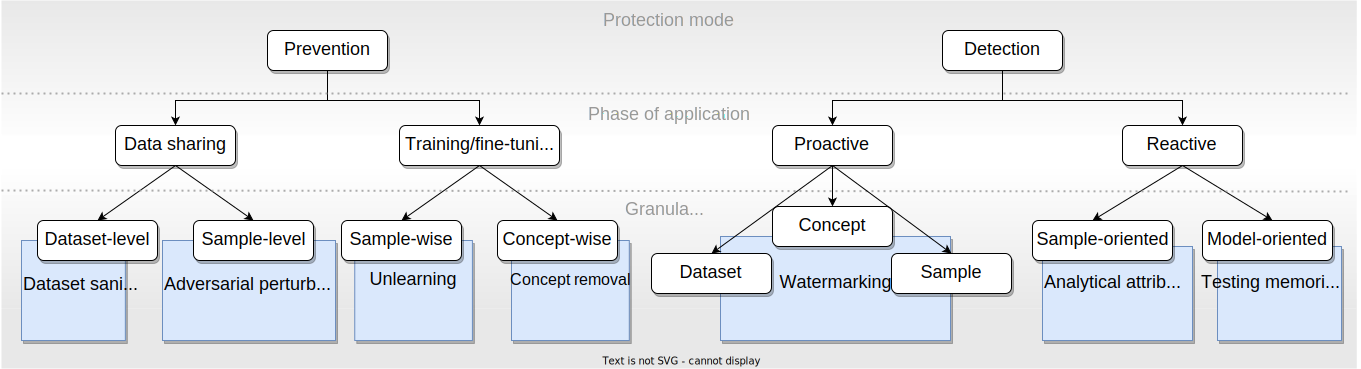
\includegraphics[width=\linewidth]{figures/taxonomy.drawio.pdf}
%     \caption{Taxonomy of IP protection methods for training data in GAI.}
%     \label{fig:taxonomy}
% \end{figure*}

\subsection{Taxonomy}\label{sec:mitigation-taxonomy}
\begin{figure*}[t!]
\begin{tikzpicture}
\node[inner sep=0pt] (taxonomy) at (0,0) {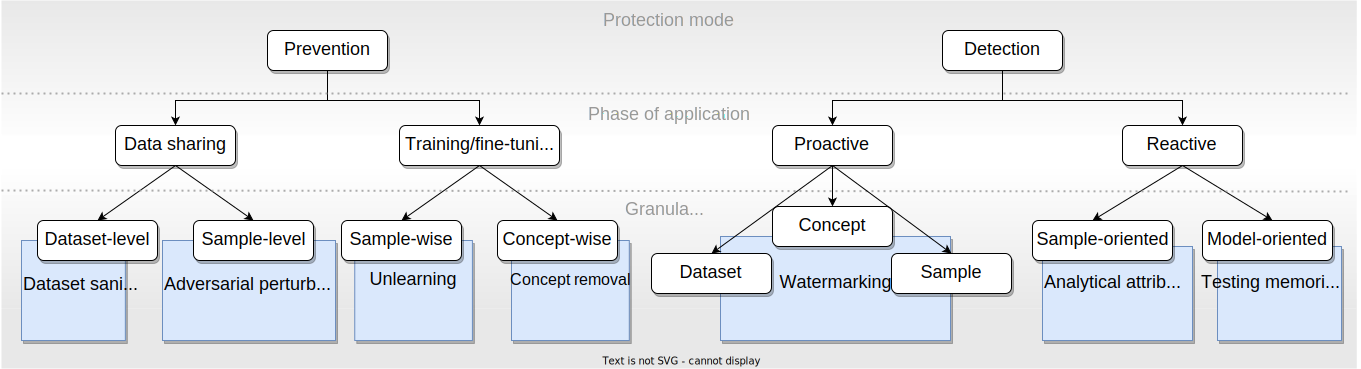
\includegraphics[width=\linewidth]{figures/taxonomy.drawio.pdf}};
% todo remove -- orientation
% \filldraw (0,0) circle (1pt);

% dataset sanitisation
\node[] (sanitisation1) at (-6.76,-0.63) {\tiny \cite{carlini_extracting_2023}};

%adversarial perturbations:
\node[] (adv1) at (-6.3,-1.60) {\tiny \cite{shan_glaze_2023,liang_adversarial_2023,liang_mist_2023,ye_duaw_2023,zhao_unlearnable_2023}};
\node[] (adv2) at (-6.32,-1.85) {\tiny \cite{chen_editshield_2023,salman_raising_2023,shan_prompt-specific_2023,zheng_understanding_2023}};
\node[] (adv3) at (-6.80,-2.1) {\tiny \cite{van_le_anti-dreambooth_2023,liu_toward_2023}};

% sanitisation
\node[] (sanitisation2) at (-4.52,-1.15) {\tiny\cite{somepalli_understanding_2023,li_mitigate_2024}};

% concept removal
\node[] (concept1) at (-3.25,-0.95) {\tiny\cite{kong_data_2023,schramowski_safe_2023,gandikota_erasing_2023}};
\node[] (concept2) at (-3.16,-1.2){\tiny\cite{gandikota_unified_2024,kumari_ablating_2023,zhang_forget-me-not_2023}};
\node[] (concept3) at (-3.40,-1.45){\tiny\cite{eldan_whos_2023,liu_rethinking_2024}};

% prompt modification
\node[] (prompt1) at (-1.65, -1.15) {\tiny\cite{somepalli_understanding_2023,noauthor_openai_2023}};
\node[] (prompt2) at (-1.6, -1.40) {\tiny\cite{hanu_detoxify_2020}};

% watermarking
% dataset-wise
\node[] (wm_dataset) at (1.0, -1.05) {\tiny\cite{cui_diffusionshield_2023}};
% sample-wise
\node[] (wm_sample1) at (2.65, -1.05) {\tiny\cite{zhang_editguard_2023,hayes_generating_2017,ma_generative_2023}};
\node[] (wm_sample2) at (2.65, -1.30) {\tiny\cite{cui_ft-shield_2023,tan_somewhat_2023,liu_detecting_2024}};
% concept-wise
\node[] (wm_concept) at (2.05,-0.50) {\tiny\cite{feng_catch_2023}};

% analytical attribution
\node[] (analytical_attr) at (5.03, -0.95) {\tiny\cite{somepalli_diffusion_2022,carlini_extracting_2023,wang_evaluating_2023,dai_training_2023}};

% testing memorisation 
\node[] (testing) at (6.85, -1.2) {\tiny\cite{carlini_secret_2019,tsai_ring--bell_2023,vyas_provable_2023}};

\end{tikzpicture}
\caption{Taxonomy of the IP protection methods for training data in GAI.}
\label{fig:taxonomy}
\end{figure*}
 
\subsubsection{Mode of protection}
Mode of protection is the categorisation based on a broader objective towards addressing IP violations. 
It includes:
\begin{itemize}
    \item Prevention -- methods that include actions taken to mitigate or avoid potential IP violations  
    \item Detection -- methods that aim to observe and identify potential IP violations after they occur
\end{itemize}
\subsubsection{Phase of application}
Protection methods may be applied at different stages of GAI lifecycle. 
For \textit{prevention} methods we differentiate:
\begin{itemize}
    \item Data sharing phase -- methods are applied to the training data in the sharing phase before they are used for training a GAI model
    \item Model training/fine-tuning -- methods are applied during model training or fine-tuning
\end{itemize}
\subsubsection{Granularity}
This categorisation distinguishes between entities in GAI process that the method is applied on to take effect in protecting the training data. 
This includes:
\begin{itemize}
    \item Dataset -- methods in this category focus on modifying the training dataset as a whole to achieve protection
    \item Sample -- IP protection is achieved by directly applying a method on the sample of interest
    \item Concept -- IP protection targets certain features representative of a concept, rather than a single input sample. A concept is an abstraction of a set of input samples that belong under the same arbitrary category; an example of a concept in IP protection context is an artistic style.
    \item Model -- methods target the model and its behaviour, without interaction with the data, to achieve the IP protection of training data
\end{itemize}

According to these three levels of categorisation, we identify 7 types of protection techniques attached to the leaf nodes of \Cref{fig:taxonomy}.
The first category is \textit{sanitisation of the training dataset} which requires direct access to the training set and modifying the underlying data before training with the goal of preventing IP violations further down the AI generation process. 
These methods and their more detailed classification are described in \Cref{sec:mitigation-sanitising}. 
Secondly, the methods may rely on different forms of \textit{adversarial perturbations}. 
The perturbations are applied to specific samples that need to be protected, and they cause the targeted behaviour in the downstream generation process. These methods are further described in \Cref{sec:mitigation-adversarial}.
Third, the \textit{unlearning} and \textit{concept removal} methods modifying the model parameters rely on re-training or fine-tuning the model, hence they require access to the training process. These are described in \Cref{sec:mitigation-concept}.
Proactive detection techniques fall under the umbrella of \textit{watermarking} and are described in \Cref{sec:mitigation-watermarking}.
Lastly, the reactive detection methods do not modify the data collection, training or generation process but can rather serve as detection of potential violations (\textit{analytical attribution}) or an indicator that the additional preventive methods should be applied (\textit{testing memorisation}). We provide details about these methods in \Cref{sec:mitigation-detection}.
% Some of these methods are specialised for certain types of models, e.g. diffusion, GANs or LLMs, etc. and differ in what type of violation is mitigated and the phase of their application. 


% Many mitigation techniques are oriented towards diffusion models and text-to-image models in general, perhaps because of the great popularity of this technology over the last few years, and ongoing criticism from the artist. Arguably, the image domain is more prone to copyright issues due to the nature of human perception towards visual art compared to, for example, language models and literary art.  
% The earlier phase of method application is content sharing. This encompasses those methods whose effectiveness relies on being applied before the content is collected for model training. 
% Those applied during \textit{training} generally rely on modifying the training data, and by \textit{fine-tuning} the weights of the model are being calibrated. Methods can be applied at the \textit{inference time}, e.g. sanitising the user prompts and finally \textit{post-hoc}, after the potential violations have already occurred.
\subsection{Classification of IP protection methods}\label{sec:mitigation-categories}
\subsubsection{Sanitising training dataset}\label{sec:mitigation-sanitising}
% deduplicating training data + image caption modification --> sanitising training data
\paragraph{Deduplicating training data} 
Current models are trained on massive datasets scraped from the internet containing billions of images. The duplicates are an issue as the search space is big and automated analysis is challenging. The problem of duplicates is prominent - for LAION-2B roughly 700 million images are reported to be duplicates~\cite{webster_-duplication_2023}.
We discussed in \Cref{sec:memorisation} that duplicated samples (e.g. more than 100 times) are easier to replicate for diffusion models~\cite{carlini_extracting_2023}, GANs and language models~\cite{carlini_extracting_2021,kandpal_large_2023}.
Deduplicating is hence a mitigation step of removing the exact or approximate duplicates from the training set with the goal of mitigating the memorisation. 
This can be done by either removing the exact duplicates or the matches found with more advanced methods such as CLIP similarity~\cite{radford_learning_2021}. 
This method is straightforward and can significantly reduce the number of replicas at inference time (e.g. \cite{carlini_extracting_2023} has shown up to a 23\% decrease in replicas for diffusion models). 
Deduplication, while not alleviating the problem~\cite{somepalli_understanding_2023}, is among the strong factors contributing to some of the memorisation behaviour.

% \textit{Undesirable image removal. Previous work to avoid
% undesirable image output in generative models has taken
% two main approaches: The first is to censor images from the
% training set, for example, by removing all people [25], or by
% more narrowly curating data to exclude undesirable classes
% of images [39, 27, 33]. Dataset removal has the disadvantage
% that the resources required to retrain large models makes it
% a very costly way to respond to problems discovered after
% training; also large-scale censorship can produce unintended
% effects [26]. The second approach is post-hoc, modifying
% output after training using classifiers [3, 21, 29], or by adding
% guidance to the inference process [38]; such methods are
% efficient to test and deploy, but they are easily circumvented
% by a user with access to parameters [43]. We compare both
% previous approaches including Stable Diffusion 2.0 [30],
% which is a complete retraining of the model on a censored
% training set, and Safe Latent Diffusion [38], which the stateof-the-art guidance-based approach. The focus of our current
% work is to introduce a third approach: we tune the model
% parameters using a guidance-based model-editing method,
% which is both fast to employ and also difficult to circumvent.}- from "Erasing concepts"

\paragraph{Image caption modification} % check if more info or papers relevant
% found very relevant one, but questioning its legitness - https://arxiv.org/abs/2309.07254
% figure
\begin{figure*}
    \centering
    \includegraphics[width=0.9\textwidth]{figures/caption-modification.PNG}
    \caption{\textbf{Caption modification}: The most successful mitigation strategies for Stable Diffusion - \textit{multiple captions} for train time and \textit{random token/number addn.} for inference time. Top column represents train samples, the middle column is the memorised image and bottom row is the generation with a mitigation strategy applied.~\cite{somepalli_understanding_2023}}
    \label{fig:caption-modification}
\end{figure*}
% why this is a mitigation strategy
The memorisation capabilities of text-to-image models are amplified by duplicated image captions alongside the duplicated training images. 
By reducing the amount of image caption duplication, the replication of training samples in generative models can be significantly reduced (even if the training image deduplication has not been performed). 

% how is it performed
In \cite{somepalli_understanding_2023} the authors propose several techniques for reducing data replication at both training and inference time by randomising and augmenting image captions in the training set. 
These strategies can be applied either at train time to increase caption diversity among duplicates, or at inference time to disrupt the memorised connection between a caption and an image. 
Namely, the strategies mentioned include:
\begin{itemize}
    \item Multiple captions - for instance, using some of the pre-trained vision-language frameworks for generating synthetic captions (e.g. BLIP~\cite{li_blip_2022})
    \item Adding a small amount of Gaussian noise to text embeddings
    \item Random caption replacement - replacing the existing caption of an image with a random sequence of words
    \item Random token replacement and addition - randomly replace words in the caption with a random word, or add a random word to the caption at a random location
    \item Random word repetition - repeat a random word from a caption at a random location of the same caption
    \item Random numbers addition - add a random number at a random location in the caption
\end{itemize}
While all proposed strategies reduce the similarity of the generated images to the corresponding training sample to some extent, for Stable Diffusion the most effective strategy is introducing \textit{multiple captions} at train time, and \textit{random token replacement/addition} at inference time, both shown in \Cref{fig:caption-modification}.

Another caption modification method was proposed in ~\cite{li_mitigate_2024}. In order to mitigate replication they generalise image captions to reduce specificity, as highly specific captions can act as keys to memory of the model. The generalisation is done by LLM, specifically GPT-3.5, guided by the prompt. 
Additionally, they further sanitise the data by combining the text embedding of the generalised caption with text embedding from another context (which is also done with the same context for corresponding image encodings). This augmentation strategy increases the diversity of the data and reportedly reduces the replication rate.

% \subsection{Input filtering}
% Input filtering as memorisation mitigation in diffusion models

% midjourney prevents the generation of known copyrighted data (Steve McCurry):\url{https://ceoln.wordpress.com/2022/12/16/some-light-infringement/}. The drawback of these filters is that they can be easily circumvented (Rando et al., Wen et al.) and the solutions are anyway just a patch and do not scale

% \subsection{Machine unlearning}
% Machine unlearning~\cite{sekhari_remember_2021,neel_descent--delete_2020,zhang_forget-me-not_2023,golatkar_eternal_2020,baumhauer_machine_2022} has firstly been proposed for addressing \textit{Right to be forgotten?} - the right to opt out of large datasets where personal data has been used without the consent of its subject. 
% The concept hence draws the motivation from user privacy protection, but has applications beyond that, e.g. erasing inaccurate or outdated information or removing harmful, manipulated data or outliers and copyright protection. 
% The aim of machine unlearning is to modify a model to behave as if specified training data has not been present, hence the list of training samples is required as an input to these methods. 
% The challenge of machine unlearning is achieving an acceptable trade-off between loss in the utility of the model and success of forgetting. 
% \textit{The possibility of such exact memorization has driven privacy and copyright concerns
% and has led to work in machine unlearning [40, 4, 15], which
% aims to modify a model to behave as if particular training
% data had not been present. 
%However, these methods are based
%on the assumption that the undesired knowledge corresponds
%to an identifiable set of training data points. The problem we
%tackle in this paper is very different from the problem of unlearning specific training data because rather than simulating
%the removal of a known training item, our goal is to erase a
%high-level visual concept that may have been learned from a
%large and unknown subset of the training data, such as the
%appearance of nudity, or the imitation of an artist’s style}-from "Erasing concepts"
% Machine unlearning has applications beyond protecting user privacy. For instance, one can use unlearning to erase inaccurate or outdated information from trained models (e.g., due to errors in labeling or changes in the environment) or remove harmful, manipulated, or outlier data.

%Forgetting concepts: Forget-me-not~\cite{zhang_forget-me-not_2023}

\subsubsection{Adversarial perturbations}\label{sec:mitigation-adversarial} % old: cloaking

\begin{table*}
    \centering
\caption{Adversarial perturbation-based protection methods and their main properties. I2I: image-to-image translation; T2I: text-to-image generation; CT2I: customised text-to-image.}
\label{tab:adversarial-perturbations}
\rowcolors{2}{white}{gray!15}
    \begin{tabular}{l|>{\raggedright\arraybackslash}p{0.19\linewidth}>{\raggedright\arraybackslash}p{0.08\linewidth}>{\raggedright\arraybackslash}p{0.23\linewidth}>{\raggedright\arraybackslash}p{0.16\linewidth}}
 \toprule
 \textbf{Method}& \textbf{Method target}& \textbf{Scenario} & \textbf{Violation} & \textbf{Distortion}\\
 \midrule
         AdvDM~\cite{liang_adversarial_2023}&  diffusion&  CT2I, I2I &  style mimicry
unauth. editing & semantic\\
         Mist~\cite{liang_mist_2023}&  VAE encoder \& diffusion&  CT2I, I2I &  style mimicry
unauth. editing& semantic/graphical \\
         UDP~\cite{zhao_unlearnable_2023}&  diffusion& T2I, CT2I &  style mimicry
unauth. training&graphical \& semantic\\
         Glaze~\cite{shan_glaze_2023}&  VAE encoder& T2I, CT2I &  style mimicry& semantic\\
         DUAW~\cite{ye_duaw_2023}&  VAE decoder& CT2I &  style mimicry
unauth. training& graphical\\
Nightshade~\cite{shan_prompt-specific_2023} & VAE encoder & T2I & unauth. training   & graphical \& semantic \\
 Anti-Dreambooth~\cite{van_le_anti-dreambooth_2023} & fine-tuning process & CT2I & unauth. training & graphical \& semantic\\ 
 Metacloak~\cite{liu_toward_2023} & fine-tuning process & CT2I & unauth. training & graphical \& semantic\\
 ACE~\cite{zheng_understanding_2023} & fine-tuning process & CT2I & style mimicry, unauth. training & graphical\\
 EditShield~\cite{chen_editshield_2023}&  VAE encoder&  I2I&  unauth. editing& semantic\\
 Photoguard~\cite{salman_raising_2023}& VAE encoder \& diffusion& I2I& unauth. editing& graphical\\
 \bottomrule
    \end{tabular}
    
    
\end{table*}
\begin{figure*}[ht]
    \centering
    \includegraphics[width=0.9\textwidth]{figures/glaze.PNG}
    \caption{\textbf{Cloaking} via Glaze~\cite{shan_glaze_2023}: columns 1-2 represent original artwork from three artists; column 3 represents the style mimicry using Stable Diffusion; column 4 is the representation of the target, "cloak" style; columns 5-6 is the attempt of style mimicry on cloaked artwork}
    \label{fig:cloaking}
\end{figure*}
IP owners can actively protect their intellectual property from GAI through a strategic application of adversarial examples. 
% what are adversarial examples? - citations. 
Adversarial examples are inputs to machine learning models deliberately designed to cause the model to make a mistake. 
They employ imperceptible changes to input data that target the learned features and decision boundaries, ultimately leading to incorrect outputs at the inference time. 
Drawing the motivation from the well-researched realm of adversarial examples for discriminative models~\cite{goodfellow_explaining_2015,zhang_adversarial_2020}, %carlini&wagner2017,adry2018 
Liang et al. introduce adversarial examples for generative models~\cite{liang_adversarial_2023}.
Unlike in classification models, where adversarial examples aim to cause misclassification, in diffusion models, they disrupt the generation process by preventing features from being extracted. 
 Such definition of adversarial examples enables direct application in safeguarding intellectual property in the domain of AI-generated content as employing adversarial perturbations can ensure that the models cannot reproduce or learn from the specific style of the protected artworks and/or cause low quality of the generated content. 
The adversarial perturbations are minimal modifications to the original images that should stay visually imperceptible. 
In different works these modifications acquired diverse terminology due to the rapid concurrent development and hence lack of standard. For instance, the modifications may be referred to as \textit{adversarial perturbations}~\cite{liang_adversarial_2023,liang_mist_2023}, \textit{adversarial noise}~\cite{zhao_unlearnable_2023}, \textit{watermark}~\cite{ye_duaw_2023}, \textit{style cloak}~\cite{shan_glaze_2023}, and the method of applying these modifications \textit{immunisation}~\cite{salman_raising_2023}, \textit{cloaking}~\cite{shan_glaze_2023} or \textit{poisoning}~\cite{liu_toward_2023}. 
 
 AdvDM~\cite{liang_adversarial_2023} is a method designed using the definition of adversarial examples for diffusion models. 
 The approach suggests utilising the training loss of diffusion models, referred to as \textit{semantic loss}, to create adversarial examples. 
 This semantic loss aims to shift the image representation away from the semantic space of the model, leading to the production of images with chaotic content when generated by the model.
 %add how optimising this loss implies targeting the diffusion process of the DM
In the subsequent work, Liang and Wu introduce Mist~\cite{liang_mist_2023}, a method that significantly improves transferability and robustness of adversarial examples across different DM applications compared to AdvDM by optimising a novel adversarial loss term, \textit{textural loss}\footnote{The authors interchangeably use textural and textual loss for describing the same loss; we believe that the correct term is textural loss as this loss exhibits modifications in \textit{textural} characteristic on the image background}. 
Textural loss represents the distance between the encoded representation of the original image and the representation of the perturbed image in the latent space of LDMs. 
The adversarial example is then generated by adding subtle perturbation to the image to maximise the textural loss. % add how optimising textural loss implies targeting the encoder and the latent representation of the input, hence it can exclusively be applied to LDMs
The method of creating Unlearnable Diffusion Perturbation (UDP)~\cite{zhao_unlearnable_2023} further increases the distortions in the generated content in order to protect images from being used for training or fine-tuning the diffusion models via adversarial perturbations. 
To achieve the unlearnable effect, the design objective is to increase the distance between the distribution of generated images and the distribution of clean training data as much as possible by adjusting the protective noise.

Glaze~\cite{shan_glaze_2023} is another method utilising minimal imperceptible perturbation to images for misleading generative models from accurately mimicking the specific artist's style. 
The perturbations are optimised to shift the image representation in latent feature space, similarly to the idea of textural loss in Mist.
Glaze, however, targets specifically the style features instead of compromising the quality of the generated output. 
This is done by firstly applying style transfer to the original art. 
Style transfer modifies the original images to adopt the appearance of a different style - the target style, while retaining the content from the original art. 
The style cloak, or the perturbation is then obtained by minimising the distance between the feature representation of the original image and the style-transferred one.
As a result, the applied perturbations are not recognisable to the human eye, but the model will generate a recognisably different style when prompted to generate art in the victim's style as shown in \Cref{fig:cloaking}. 

A more universal approach to creating adversarial perturbations that protect copyrighted images is proposed by the authors of Data-free Universal Adversarial Watermark (DUAW)~\cite{ye_duaw_2023}. 
DUAW disrupts the variational autoencoder in Stable Diffusion models, ensuring that images altered by the adversarial perturbation (here called a watermark) produce significantly distorted outputs when used for model customisation.
%(such as DreamBooth~\cite{ruiz_dreambooth_2023} and LoRA~\cite{hu_lora_2021}). 
Hence, this method, besides rendering the artistic style unrecognisable, also disrupts the model as a result of the unauthorised usage of the copyrighted input. 
Unlike the previous methods, DUAW operates without direct access to the copyrighted images, using synthetic data for optimising the adversarial perturbation instead. 
Nightshade~\cite{shan_prompt-specific_2023} takes a step further into degrading the quality of the generated output from a text-to-image model as an overall goal of this method is to prevent training on unauthorised data and serves as a strong disincentive to disregard the copyright notices and opt-out choices. 
The authors first demonstrate that despite the massive datasets used in training diffusion models, they are vulnerable to poisoning attacks targeting specific prompts. 
The method relies on this observation and uses a small number of visually identical poison samples to corrupt the response of a model to specific prompts. 
The protection method shows large effects on related concepts and hence destabilises general features in the model, affecting its overall image generation ability.

Anti-DreamBooth~\cite{van_le_anti-dreambooth_2023} and MetaCloak~\cite{liu_toward_2023} are black-box approaches based on training surrogate models to optimise the perturbations, where the objective is to force the target model to overfit on these perturbations in the fine-tuning stage. These methods are designed specifically for the unauthorised CT2I scenario.

Adversarial perturbations have shown to be effective against unauthorized instruction-guided image editing
%(e.g. techniques such as Instruct-Pix2Pix~\cite{brooks_instructpix2pix_2023}) 
by ensuring that images manipulated with instruction-guided DMs result in unrealistic outcomes~\cite{chen_editshield_2023,salman_raising_2023}. 
While copyrighted images and artworks may be subject to such edits, unauthorised editing implies a broader range of misuse, such as privacy issues and spreading misinformation. % maybe some citation here
In terms of intellectual property, these methods protect the integrity of the original work. 
Photoguard~\cite{salman_raising_2023} introduces two types of protection methods; (i) \textit{encoder attack} and (ii) \textit{diffusion attack}.
Encoder attack perturbs the input image such that the VAE of LDM maps the image to a wrong representation in the latent space, e.g. representation of a target image which can be random noise, however, the generated image usually preserves the information from the textual prompt.
Diffusion attack aims to perturb the input image so that the \textit{final} image generated by the LDM is a specific target image (e.g. random noise), hence targeting the full diffusion process which includes the text prompt conditioning.
Although the diffusion attack generates the images closer to the target image, it is very computationally expensive as the optimisation of the perturbations requires backpropagation through the full diffusion process.
EditShield~\cite{chen_editshield_2023} employs an encoder attack without a specific target image. Instead, the approach is to maximise the distance of the perturbed representation from the original representation while constraining the amount of perturbations to keep them visually imperceptible. 
They further introduce a method for finding universal perturbations for unauthorised image editing that can protect a large amount of images without a repetitive process of finding the optimal perturbation for each image.  	
% todo: MetaCloak and ITA --> fall under this category but do not have citations

Adversarial perturbation-based methods and their main properties are summarised in \Cref{tab:adversarial-perturbations}. 
We outlined the \textit{method target}, i.e. the part or the sub-process of a generative model that the adversarial modifications affect.
The resulting \textit{distortions} in the generated content can be observed as two main types. Firstly, the \textit{semantic distortions} render the objective of a malicious action ineffective, while keeping the overall quality high. 
For instance, keeping the content of an image while not adhering to textual prompt requesting a specific style of the generated image. 
Secondly, \textit{graphical distortions} compromise the perceptual quality of the generated image.

The main challenge of protecting against style mimicry via adversarial perturbations is directing these perturbations such that they shift specifically those features related to the artistic style of the victim, i.e. achieving only semantic distortions, as the artistic style is very hard to be formally defined. 
Glaze addresses this issue by employing their style-transfer trick to target only the style features, while other methods come with the cost of degrading the quality of the generated output (quality distortion).
However, this cost can be seen as a desired consequence as it provides an additional layer of protection. 
Larger disruptions in the generated content cover the broader range of violations, specifically, they protect against the unauthorised usage of copyrighted images in the training process. 
The protection is especially effective in scenarios of fine-tuning the diffusion models (style transfer scenario) where the protected imagery has a more direct impact on the generated content~\cite{liang_mist_2023}.
All methods, to take effect, need to be applied to images before their usage in the model, whether it is the training or customisation and editing. 
This means that the responsibility of protection is laid on IP owners to apply these methods during the sharing phase.
This entails two challenges for effective and sustainable protection: (i) the level of awareness and education needs to be significantly increased to encourage the intellectual property owners (usually an artist) to apply these methods when sharing their work online, and (ii) the GAI provider can rather easily circumvent the protective effects of adversarial perturbations with the release of new versions of generative models. 
These can be addressed by shifting the responsibility to other stakeholders such as hosting platforms and AI providers and their collaboration. 
As discussed in \cite{salman_raising_2023}, one instance of such collaboration may involve the AI provider offering the cloaking/immunisation APIs for their models and ensuring their forward compatibility with future versions.

%\reminder[inline]{Adversarial examples for GANs (or other generative models in other domains) -- is there an evaluation on IP protection? If not, then just mention the techniques.}

%\reminder[inline]{Notable mentions: papers that highly inspired the work in this category but do not evaluate on IP protection scenario. Such as Anti-DreamBooth - optimising adversarial wm to disrupt the diffusion process, preventing the representation learning process}
% e.g. "Erasing concepts" paper compares their methods to SDM

\subsubsection{Concept removal and unlearning}\label{sec:mitigation-concept}
\begin{figure*}[ht]
    \centering
    \includegraphics[width=0.9\textwidth]{figures/erasing-concepts.png}
    \caption{\textbf{Concept removal}: images generated without and with \textit{erasing concepts} method~\cite{gandikota_erasing_2023}}
    \label{fig:erasing-concepts}
\end{figure*}
\begin{figure*}[ht]
    \centering
    \includegraphics[width=0.9\textwidth]{figures/ablating-concepts.jpg}
    \caption{\textbf{Concept removal}: images generated without and with applying \textit{concept ablation}~\cite{kumari_ablating_2023}}
    \label{fig:ablation}
\end{figure*}
Earlier works that addressed the memorisation of exact objects, text embeddings etc. in large generative models focused on the persistence of harmful elements from the training set that reflect in the generated data, such as violence and sexual content. 
Cleansing the test set from harmful samples and retraining the model from scratch does not practically work for large models already pre-trained on large data. Furthermore, censoring concepts at inference time is shown to be easy to bypass~\cite{rando_red-teaming_2022}.
The effective mitigation techniques in this category primarily focus on concept removal via fine-tuning, although some proposed techniques require at least a fraction of full retraining with the benefit of removing undesirable samples. 
For instance, the authors of \textit{data redaction}~\cite{kong_data_2023} method aim to remove data from pre-trained GANs by re-training the model on the original set, adding the redacted data to the fake data set and applying standard adversarial loss. 
%Although they do not specifically show that the method can be used for IPR protection, but rather focus on debiasing the data and improving model quality, we claim that the method could be used to remove targeted samples from the model, hence providing an opt-out option. (??) % todo: verify that this fits under "concept removal"
Furthermore, \textit{Safe latent diffusion}~\cite{schramowski_safe_2023} is proposed as a version of the Stable Diffusion (SD) model, trained to exclude inappropriate imagery originally contained in the LAION dataset used to train the SD. Hence, the work is focused on removing harmful and offensive concepts such as hate, harassment, sexual content, self-harm, violence, shocking images, and illegal activity, although it is noted that the method can be used to remove any specified concept.
%performs image editing at inference (post-hoc) without any further fine-tuning. 
% The work is focused on removing harmful and offensive concepts such as hate, harassment, sexual content, self-harm, violence, shocking images, and illegal activity, although it is noted that the method can be used to remove any specified concept and the authors encourage transparency about which concepts are being removed.
% This version of Stable Diffusion is trained to exclude harmful imagery, such  as violence... 

% For
% Safe Latent Defusion, the authors focus on removing inapropriate concepts such as violence and
% nudity while Kumari et al. focus directly on mimicking artistic styles, hence provide a technology for opt-out
% option for artistis whose art is already contained in the training data of the pretrained models.

% Furthermore, \textit{Safe latent diffusion}~\cite{schramowski_safe_2023} performs image editing at inference (post-hoc) without any further fine-tuning. The work is focused on removing harmful and offensive concepts such as hate, harassment, sexual content, self-harm, violence, shocking images, and illegal activity, although it is noted that the method can be used to remove any specified concept and the authors encourage transparency about which concepts are being removed.
% This is a version of Stable Diffusion trained to exclude harmful imagery, such  as violence... 

Fine-tuning methods for pre-trained models, on the other hand, need significantly less computation time to tackle the problem of removing concepts.
The goal is to remove the target concept permanently from the model by modifying its weights while minimising the effects on other concepts.
% \textit{Erasing concepts}~\cite{gandikota_erasing_2023} proposes a method for concept removal via fine-tuning model weights, hence removing the concept permanently rather than just at the inference time like its predecessor(??). 
%Given the text description of the target concept, the method can modify the model weights to erase the concept while minimising the effects on other concepts. 

In \cite{gandikota_erasing_2023}, \textit{erasing concepts} is based on the observation that cross-attention modules serve for text conditioning in text-to-image models (as opposed to self-attention modules that activate regardless of the text conditioning), therefore by fine-tuning these parameters the connection between text prompts and the output images can be removed. 
\Cref{fig:erasing-concepts} shows how this method can be scaled to remove harmful concepts or unwanted objects and mitigate style mimicry attacks.
Unified concept editing (UCE)~\cite{gandikota_unified_2024} is a generalised method from the same group of authors, who in this work combine resolving the issues of style mimicry, bias and offensive content by concept erasure while causing minor effects on other concepts.   

Other fine-tuning-based approaches~\cite{kumari_ablating_2023,zhang_forget-me-not_2023} propose \textit{concept ablation}/\textit{concept unlearning} by directing the unwanted samples towards a more general concept.
These methods require additional input from the user - the description of a generalised concept in relation to the target concept - the \textit{anchor concept}. 
During fine-tuning, the objective is to teach the model to generate the output as if the anchor concept was prompted instead of the target concept (e.g. "Nemo leaping out of the water" as "A fish leaping out of the water") via minimising the statistical distance between the target concept generated image distribution and anchor concept image distribution. 
The resulting ablated images shown in \Cref{fig:ablation} lose the specific features of the target concept. 
Some limitations noted in this paper include the degradation in closely surrounding concepts (e.g. ablation of the concept "Van Gogh" highly affects the concept "Monet").
% Although the general style mimicking mitigation is not scalable using this method, it provides a promising underlying technology for artists to opt out of the huge pre-trained diffusion models. 
These concept removal techniques for image generation are shown to be useful for the mitigation of style mimicry as the artistic style could in this sense also represent a concept. 
This paves the way for developing efficient opt-out techniques for artists who wish to secure their works against mimicry. 

Unlearning techniques for LLMs include algorithms for approximating the removal of training data without retraining the model which would be infeasible. 
Two objectives are usually addressed in LLM unlearning - \textit{model capability removal}, mostly relevant for achieving privacy and safety and \textit{data influence removal}, crucial for intellectual property protection~\cite{liu_rethinking_2024}
For generative models, the methods usually evaluate the privacy and safety scenarios~\cite{jang_knowledge_2022,wu_depn_2023,lu_quark_2022}, while a few address intellectual property use case.
One such method demonstrates a case study using "Harry Potter" as a targeted content~\cite{eldan_whos_2023}. It proposes generating generic predictions to replace specific content, thereby the memory of the targeted information while preserving its general performance. 
In-context unlearning~\cite{pawelczyk_-context_2023} is a black-box unlearning method without direct access to the model parameters. This method uses flipped labels and additional correctly labelled instances at inference time to eliminate the influence of a training point on the model output.

\subsubsection{Watermarking \& ownership verification}\label{sec:mitigation-watermarking}
% ad-hoc verification of participation; watermarking; ownership verification
\begin{figure}
    \centering
    \includegraphics[width=\linewidth]{figures/watermarking-stages.PNG}
    \caption{The two stages of forensic watermarking~\cite{cui_diffusionshield_2023}.}
    \label{fig:watermarking-stages}
\end{figure}
Watermarking methods for content subject to unauthorised usage as training data of generative models involve embedding imperceptible signals or patterns into the content to assert ownership, trace unauthorised use and protect intellectual property. 
These techniques ensure that any content generated by AI that leverages such watermarked data can be identified or verified as originating from protected sources, providing a mechanism for creators (copyright owners, artists, etc.) to safeguard their work. 
Unlike the methods based on adversarial noise, the watermarking methods do not sacrifice the utility of the protected images for generation purposes but rather enable passive protection based on detecting or verifying data ownership. 
For example, those watermarking methods addressed in \Cref{sec:mitigation-adversarial} exhibit this exact difference. 
In \cite{zhang_editguard_2023} the authors refer to these as \textit{adversarial} watermarks as opposed to \textit{forensic} watermarks which are covered in this section. 
Forensic watermarks are achieving the goals of ownership verification and traceability. 
This implies a two-stage process of forensic watermarking which is another key property of this class of methods as depicted in \Cref{fig:watermarking-stages}. 
The methods generally consist of (i) the \textit{protection stage} where the watermark is being created and embedded into the training samples; this stage takes place before content sharing and (ii) the \textit{audit stage} which includes detecting the watermark from the generated content, its verification and further actions due to the committed violations. 
Forensic watermarking has the following main requirements:
\begin{itemize}
    \item \textit{robustness} -- watermark is robust to changes in the content caused by the generation process or a text-guidance
    \item \textit{fidelity} -- a.k.a \textit{invisibility}; watermark causes little impact on the quality of both the input (protected) samples and generated/synthesised output
    \item \textit{effectiveness} -- successful watermark extraction from the watermarked content
    \item \textit{integrity} -- a valid watermark cannot be extracted from a non-watermarked content
\end{itemize}

% Watermarking GANs
Watermarking has been proposed for GANs~\cite{hayes_generating_2017}. 
The scheme for embedding a secret message within an image is based on adversarial training of three neural networks, A, B and C. 
A embeds a secret message within the original unmodified, \textit{cover} image, producing a \textit{steganographic} image and sends it to B who can recover the message. E can eavesdrop on the link between A and B and aims to discover if there is a secret message embedded within their communication, hence, given an image, E places a confidence score of how likely the image is cover or steganographic. 
Given this scenario, network A is learning to embed a message such that network B can recover it and network E can do no better than randomly guessing if an image is a cover or steganographic. 
GAN watermarking techniques require full access to the training process and perform no better than random guessing for subject-driven synthesis which is common for diffusion models~\cite{ma_generative_2023}. 

For diffusion models, GenWatermark~\cite{ma_generative_2023} is a watermarking method for protecting image data in a subject-driven synthesis scenario. 
The method consists of a generator and a detector, both pre-trained on a large general dataset and optimised in an adversarial learning manner under the bound of perturbation budget; the generator is learned to generate strong watermarks while the detector learns to distinguish between clean and watermarked images. 
This concludes the first phase, after which, a generator and a generic detector are trained. 
In the second phase, the detector can be fine-tuned to a specific subject (e.g. one artistic style). 
This is done such that two models are trained, a clean model on a clean image set and a watermarked model on a corresponding watermarked image set. 
These two models are then used to synthesise image sets for fine-tuning the detector.
Similarly, concept watermarking~\cite{feng_catch_2023} is proposed with a similar idea of jointly training a watermark encoder and watermark decoder to embed a watermark into a specific concept. 
This method is evaluated specifically for a textual inversion scenario, i.e. subject-driven fine-tuning, hence the watermark is directed towards the introduced word.   
FT-Shield~\cite{cui_ft-shield_2023} is another method designed for fine-tuning text-to-image diffusion models. 
The perturbations that represent a watermark are optimised such that they are learned by the diffusion model before other features such as style.
Watermark detection is done by a binary classifier learned on to distinguish clean from watermarked images using the original pairs of clean and protected images and augmented with images generated by the model. 

DiffusionShield~\cite{cui_diffusionshield_2023} is a method that embeds visually imperceptible watermarks into images and ensures that the watermark is learned by a diffusion model and reproduced in generated images, allowing the detection of a legitimate owner.
The watermark hence persists in the diffusion process unlike prior image watermarking approaches based on the frequency domain~\cite{navas_dwt-dct-svd_2008} and NNs~\cite{zhu_hidden_2018} and those designed for DeepFake detection~\cite{yu_artificial_2021}.
The authors assume a scenario where the data owner has rights over multiple images and embeds the same watermark into each of them. 
The effectiveness of the watermarks is also demonstrated for scenarios where multiple owners embed separate (different) watermarks into their respective images. 
EditGuard~\cite{zhang_editguard_2023} proposes the framework achieving two goals simultaneously; copyright protection and tamper localisation. 
It leverages image-into-image steganography (an image embedded within another image) for embedding and accurately decoding both tampered areas and copyright information. 
Robust Invisible Watermarking (RIW)~\cite{tan_somewhat_2023} is a watermarking technique specifically designed for unauthorised editing. 
Watermarks are typically simple, repetitive images such as plain text with a black background and are embedded into the latent representation of the target image. 
This method optimises the watermark separately for each input sample. 
After editing, the watermark can be extracted by calculating a pixel-wise difference between the watermark and the edited image or utilising an OCR (Optical Character Recognition) model, the latter being more effective.

TimbreWatermarking~\cite{liu_detecting_2024} is a method for watermarking against unauthorised audio synthesis. 
It embeds a watermark in the frequency domain that aims to be detectable after voice cloning attempts.
%todo 
% \reminder[inline]{
% Related: Marking for detecting deepfakes (generated content detection, e.g synthID, \cite{fernandez_stable_2023,wen_tree-ring_2023}), authenticity verification (checking a potentially manipulated watermark) 
% }

\subsubsection{Detection and attribution}\label{sec:mitigation-detection}
% Detection: the premise is that we don't know whether the sample is part of the training data
% Attribution: the premise is that we know that the sample is part of the training set
\begin{figure}
    \centering
    \includegraphics[width=\linewidth]{figures/attribution.PNG}
    \caption{Attribution by Customisation (AbC)~\cite{wang_evaluating_2023}}
    \label{fig:attribution}
\end{figure}

To provide the artists an efficient and rather quick way to make initial steps in protecting their art, efforts have been put into developing tools where artists can verify whether their art is part of large datasets and consequently, a part of training sets for generative models, i.e. the \textit{detection of participation}. 
One such solution is a project \textit{Have I been trained?}\footnote{\url{https://haveibeentrained.com/}} %~\cite{noauthor_have_nodate} 
by a company \textit{Spawning} \footnote{\url{https://www.spawning.ai}}. %~\cite{noauthor_spawningai_nodate}. 
The tool relies on CLIP retrieval to enable artists to search LAION-5B and LAION-400M datasets that are used to train Stable Diffusion and Midjourney models. 
In the Spawning framework, this detection serves as an initial step which can be followed by an opt-out mechanism for artists to retract their art from the datasets. 
%Spawning automates the process of identifying and flagging non-consenting data, creating opt-out lists that are forwarded to LAION who have agreed to remove those images from its dataset~\cite{noauthor_how_2023}.

\textit{Data attribution} in generative models involves identifying the contribution of specific data samples to the generated outputs. 
From an ethical point of view, this process is crucial for understanding how models generate content, addressing not only concerns about copyright but also data privacy and transparency. 
Techniques for data attribution may include ad-hoc methods such as embedding watermarks in the training data which can later be detected in the generated content, i.e. forensic watermarks discussed in \Cref{sec:mitigation-watermarking}. 
On the other hand, different analytical methods may be used to trace the influence of training samples on the behaviour of the model. 
% We refer to these as post-hoc detection methods as they do not involve active action of any stakeholder during the data sharing or model training phase, but are rather applied after inference.

%% Membership inference applied to detect training data 

Given the generated sample, finding the matches across the large training dataset is infeasible, however, in some special cases, the approximate matches can be extracted.
This special case requires generated content to be highly, almost 100\% influenced by a single training sample and is shown to be a feasible scenario~\cite{carlini_extracting_2023,somepalli_diffusion_2022}. 
In \Cref{sec:IPR-threats} we discussed this as a data replication problem that may be leveraged for copyright infringements. 
In this context, it can serve as evidence to the copyright owner that their data has been used for training. 
When it comes to attribution in the more general, but complex scenario where the generated sample is influenced by multiple training samples, Wang et al.~\cite{wang_evaluating_2023} take a leap towards understanding the influences of an individual image in the generative process (\Cref{fig:attribution}). 
Drawing from the observations that the main challenge in attributing generated images to the training samples is the lack of ground truth for such task, the key idea is to simulate ground truth directly by adding exemplar influences.
They use textual inversion to customise images, creating this way the set of synthesised images influenced by their corresponding exemplar image. 
Using the dataset, the method tunes the retrieval feature spaces CLIP~\cite{pizzi_self-supervised_2022}, DINO~\cite{caron_emerging_2021}, ViT~\cite{dosovitskiy_image_2021}, ALADIN~\cite{ruta_aladin_2021}, SSCD~\cite{pizzi_self-supervised_2022} via contrastive learning~\cite{oord_representation_2019} to enable obtaining attribution scores representing the influence of multiple candidate images on the generated image.
In \cite{dai_training_2023} the authors introduce the \textit{encoded ensemble} method that enables identification of influential training examples by leveraging ensemble training on carefully engineered splits of the training data. 
The main limitation of this method is its computational expansiveness as it requires training ensembles of 10-50 diffusion models.

\subsection{Policy, ethical usage and recommendations}\label{sec:mitigation-ethical} % Policy-driven frameworks?
% generally here we have:
% % consent options on different platforms
% % blocking scraping 

% this section focuses on artists' options to take action
Very powerful models are already trained on a large corpus of data scraped from different sources such as portfolio sites for artists (Pinterest, ArtStation) and shopping sites (Fine Art America) without artists' consent for their art to be part of the training data.
%In particular, Stable Diffusion has been trained on the LAION-5B dataset, currently the largest image-text dataset in the world~\cite{schuhmann_laion-5b_2022,noauthor_laion-5b_nodate}

Spawning automates the process of identifying and flagging non-consenting data, creating opt-out lists that are forwarded to LAION who have agreed to remove those images from its dataset~\cite{wu_how_2023}.
Besides the efforts originating from the cooperation of Spawning and LAION regarding creating opt-out lists and removing them, mentioned in \Cref{sec:mitigation-detection}, opt-out options have recently been adopted by online artist communities such as \textit{Deviant Art}. With this, they attempt to disallow third parties to scrape the content for AI development purposes without artists' knowledge and permission~\cite{wiggers_deviantart_2022}. In fact, a default setting for artists is an \textit{opt-out}, therefore an artist needs to make an active choice and consent to opt in. 
Some platforms even prevent the scraping completely; The Guardian, New York Times, CNN, Australian Broadcasting Corporation, British Broadcasting Corporation and Reuters have reportedly blocked ChatGPT (GPTBot) and Common Crawl from scraping their content due to the intellectual property considerations of the authors and licence fee payers~\cite{bogle_new_2023,marcus_generative_2024}.
%ethical usage
% focus on end-user action
% consent-driven AI tools
Some projects address the development of ethical tools for generating art content. 
These AI tools are trained explicitly on data for which consent was given.
Spawning offers an API for training ethical models ensuring that all underlying data has been provided with consent.
One instance of a consent-respecting AI model is Holly+\footnote{\href{https://holly.mirror.xyz/54ds2IiOnvthjGFkokFCoaI4EabytH9xjAYy1irHy94}{https://holly.mirror.xyz/}}%~\cite{herndon_holly_nodate}
, a tool which allows uploading a polyphonic audio track and generating a version of it sung by a \textit{deepfake} of its creator, Holly Herndon.
% standards
% Source+ (a product of the organisation Spawning. Spawning also created "Have I been trained") -- source for this is missing, it is in beta stage apparently
\textit{Content Authenticity Initiative} are developing an open standard and provenance tool that would prove the authenticity of digital content via watermarking. 
It promotes trustworthiness and transparency by helping fight disinformation as well as protecting IPRs of digital content creators\footnote{\url{https://contentauthenticity.org}}.%~\cite{noauthor_content_nodate}. 
%OpenAI updated content policies to prohibit generating copyrighted characters, trademarks or IPs that could infringe the rights,  such as characters from movies, TV shows, books, video games, and other media. 

% ethical development
A responsible act from the perspective of model development is taking into account the concerns of memorisation and assessing the necessity of further actions (e.g. applying techniques from previous sections) before deploying the model.
It is generally a good recommendation to test the model's generalisation ability, however, this is not a good enough indicator of whether the model still memorises the training data. 
The authors in \cite{carlini_secret_2019} propose a strategy for testing the model memorisation already at training time. This can be done by augmenting the training process with some random unexpected input and measuring the likelihood of its generation. Although this method has been empirically evaluated on large text models to measure the model's potential unintended memorisation of unique sequences (e.g. Google uses it for the autocomplete), it could be repurposed for copyright protection too. 
Ring-A-Bell~\cite{tsai_ring--bell_2023} is a red-teaming framework proposed for prompt-based concept testing that generates prompts leading to the generation of problematic concepts.

Formalisation of the problem of intellectual property protection in AI is addressed in the recent work ~\cite{vyas_provable_2023}. 
The authors draw parallels from differential privacy and provide a formal guarantee on the (lack of) similarity between the output of a generative model and any potentially copyrighted data in its training set. 
The method to achieve the guarantee is evaluated on a transformer and diffusion model although it is claimed as model-agnostic.

%\section{Cost of mitigation}% implications
%todo: protection vs utility discussion
% -- differences in distortions caused by protection in levels: non-distorting (watermark), somewhat distorting (i. distorting the targeted style, ii. distorting the targeted style and related concepts; cloaking; concept removal; how much the distortion bleeds to related concepts e.g.) and distorting (poisoning)

% sections "IPR in other parts of GenAI" and "Other issues in GenAI" can be a part of related work
% in that case put the related work at the end
% Related work subsections:
% % i) Surveys
% % ii) IPR of other parts of GenAI
% % iii) Related issues in GenAI
%\section{IPR and generated content} % + IPR of models + IPR of prompts

% todo: discussions of IPR for generated content; watermarking as a protection method
% this is potentially out of scope, although it could be included just from the technical perspective and avoid the legal discussions that are anyway already in some surveys

% \section{Related issues}

% \subsection{Other recommendations}

% \paragraph{Testing model memorisation}
% \cite{carlini_secret_2019}
% The strategy is: train the model, augment the training process with some random unexplected input, ask how likely 

% Exposure metric
% Canary; likelihood (Google uses this)
% a, this paper
% introduces a quantitative metric of exposure. This metric can
% be applied during training as part of a testing methodology
% that empirically measures a model’s potential for unintended
% memorization of unique or rare sequences in the training data.

% TODO: add stakeholders as a discussion point; possibly also an axis in the taxonomy
\section{Discussion}\label{sec:discussion}
The rapid development of GAI sparked a lot of ethical debates besides those regarding intellectual property. 
For instance, the unfiltered training data and manipulative intents can lead to the generation of harmful content, including misinformation, deepfakes, imagery of violence and sexual content. 
One of the methods addressing this is concept removal and unlearning. 
Many of the proposed methods are also directly addressing style mimicry as discussed in \Cref{sec:mitigation-concept}. 
We hypothesise that the remainder of work in the area of unlearning~\cite{wu_erasediff_2024} and concept removal~\cite{schramowski_safe_2023,tsai_ring--bell_2023,liu_geom-erasing_2023,ho_classifier-free_2022} can also be utilised in the IP protection scenario by treating the artistic style as a concept. 
Furthermore, the idea behind detection-based methods that aim to remove harmful content by filtering it through safety checkers~\cite{rando_red-teaming_2022} could be repurposed for addressing copyright issues, filtering for instance art-related content.
Similarly, there are notable cloaking methods~\cite{shan_fawkes_2020} that do not explicitly evaluate on the IP protection scenario but are a valuable motivation for the methods in \Cref{sec:mitigation-adversarial}.

Membership inference (MIA) is the type of attack where the aim is to determine whether a specific data point was used in training a model. 
This can compromise privacy but can also evaluate the privacy leakage of a model. 
There is work proposed for MIA on GANs~\cite{webster_this_2021,hayes_logan_2018} and diffusion models~\cite{matsumoto_membership_2023,hu_membership_2023}. 
In the context of intellectual property protection, MIA could serve as a first line in detection of unauthorised use of copyrighted content alongside the methods discussed in \Cref{sec:mitigation-detection}. 
% \subsection{Related concerns}
% Privacy, membership inference, harmful content removal, authorship, detection of generated content, attribution...

Detection of generated content plays an indirect role in intellectual property protection, especially when it comes to creative works. 
The existing detection techniques for AI-generated text however struggle with reliability due to large false negative rates~\cite{sadasivan_can_2024,weber-wulff_testing_2023}. Moreover, the effectiveness significantly decreases when faced with machine translation and obfuscation techniques.
Similarly, passive detection techniques relying on statistical artefacts are not effective for images either~\cite{corvi_detection_2023}.
For image data, there are active watermarking techniques proposed designed to be embedded into the content to later be detected in the generated content~\cite{zhu_hidden_2018,zhang_udh_2020}, or further, attributed to a specific generative model\footnote{\url{https://deepmind.google/technologies/synthid/}}.%~\cite{noauthor_synthid_2023}.
These techniques have also shown to be insufficiently robust against minor perturbations~\cite{jiang_evading_2023}. 

% \subsection{IPR of other entities in GenAI}
% Intellectual property protection appears as an issue in the entire ecosystem of Generative AI. 
While this survey reviews the methods for safeguarding the data exposed to the training of generative models, there is an ongoing discussion and a body of research that addresses IP of other entities in the GAI ecosystem, including generated content~\cite{chesterman_good_2023} and models~\cite{ong_protecting_2021,peng_are_2023}. 
There is no consensus on who (if anyone) should own the AI-generated content, whether it is the AI provider, the user who prompted the AI or AI itself. 
So far, copyright protection has notably been denied for the artists that included prompting AI in the process of creation, such as the prize-winning “Théâtre D’opéra Spatial” by Jason M. Allen~\cite{roose_ai-generated_2022} and "A Recent Entrance to Paradise" by Stephen Thaler~\cite{brodkin_us_2023} claiming that prompting alone is not enough to claim authorship as the user has limited control over how AI systems interpret and generate the end-result. 
However, the real interaction between the user and the AI is more complex -- the generated outputs in question are usually a result of many sequential prompts and a mix of other artistic techniques such as photography, oil painting etc. 
Therefore the open question remains -- how much human input is necessary for the AI user to be qualified as an author. 
The authorship questions naturally imply the problems about the transparency of AI-generated content. 
Approaches for detecting the AI-generated content exist, for example for the AI-generated text, but are not sufficiently robust against paraphrasing and other modifications~\cite{sadasivan_can_2024}. 
Another option is to \textit{actively} embed a robust watermark carrying information about the AI that generated the content, such as SynthID.%~\cite{noauthor_synthid_2023}. 
Watermarking techniques have also been proposed for protecting the IP of the models~\cite{ong_protecting_2021} as they can be a target of \textit{model extraction} attacks (a.k.a. \textit{model stealing}) where the attacker attempts to maliciously approximate target model.
Although there have been some successful imitations of LLMs in terms of style, such as LLaMA~\cite{touvron_llama_2023}, these models are critiqued for their decreased factuality compared to the original models~\cite{gudibande_false_2023}.


\section{Conclusions}\label{sec:conclusion}
In this paper, we reviewed the potential IP violations of the training data of GAI and the state-of-the-art technical protection methods.
The reviewed methods generally achieve a few goals in terms of protection; they may limit the usability of the data samples in the training process, provide traceability and attribution of the usage of data from the generated content, protect the artistic styles from being learned and generated by the model, and detect whether particular data was a part of model training.   

% It is essential for individuals and organisations involved in generative AI to be aware of the potential violations and ensure that they have the necessary rights and permissions for the data, content, and algorithms used in the development and application of these models. 
%Seeking legal advice and adhering to intellectual property laws and regulations can help prevent such violations and protect both creators and users of generative AI models.

\bibliographystyle{ieeetr}
% \bibliography{references_Zotero} % --> uncomment for the final version
\bibliography{references-Tanja-workingVersion}  

\end{document}